\section{Assiomi di probabilit\'a e RV}

\begin{frame}{Assiomi probabilit\'a Kolmogorov e definizioni}
\begin{itemize}
	\item Assiomi di probabilit\'a: i) La probabilit\'a di un evento \'e $\prob{(E)}\geq0$ per ogni $E\in S$ spazio campionario.
	ii) La probabilit\'a degli eventi del sample space \'e 1.
	iii) $\sigma$-additivit\'a: per ogni sequenza numerabile di insiemi disgiunti (eventi mutualmente esclusivi) $\prob{(\cup_{i=1}^{\infty}E_i)}=\sum_{i=1}^{\infty}\prob{(E_i)}$
	\item Addition rule: probability that A or B will - $\prob{(A\cup B)}=\prob{(A)}+\prob{(B)}-\prob{(A\cap B)}$
	\item Probabilit\'a condizionata $\prob{(B|A)}=\frac{\prob{(B\cap A)}}{\prob{(A)}}$
	\item Teorema di Bayes $\prob{(A|B)}=\frac{\prob{(B|A)}\prob{(A)}}{\prob{(B)}}$
	\item eventi indipendenti $P(A|B)=P(A)$
\end{itemize}
\end{frame}

\begin{frame}{Distribuzioni di probabilit\'a - Convergenza di RV}
\begin{itemize}
\item Distribuzione di probabilit\'a cumulante e pdf: 	$F(x)=P(x_n<x)=\int_{-\infty}^xf(x')\,dx'$: $f(x)=\TDy{x}{F(x)}$
\item $\alpha$-point, quantile of order $\alpha$: $F(x_{\alpha})=\alpha$
\item Eventi congiunti - Probabilit\'a $([x,x+dx],y)=(A)$: marginal pdf for x $\prob{(A)}=\int f(x,y)\,dxdy=f_x(x)\,dx$, $(x,[y,y+dy])=(B)$.
$\prob{(A\cap B)}=f(x,y)\,dx\,dy$
\item Probabilit\'a condizionata $\prob{(B|A)}=\frac{\prob{A\cap B}}{\prob{A}}=\frac{f(x,y)\,dx\,dy}{f_x(x)\,dx}$; conditional pdf for y given x $h(y|x)=\frac{f(x,y)}{f_x(x)}$, simile per $g(x|y)=\frac{f(x,y)}{f_y(y)}$
\item T Bayes $g(x|y)=\frac{h(y|x)f_x(x)}{f_y(y)}$
\item law of total prob.: $f_x(x)=\intsinf{}g(x|y)f_y(y)\,dy$
\end{itemize}
\end{frame}

\section{Cambio di variabile: come cambia pdf?}

\begin{frame}{Trasformazione pdf per cambio variabile}
\begin{figure}\
	\centering
	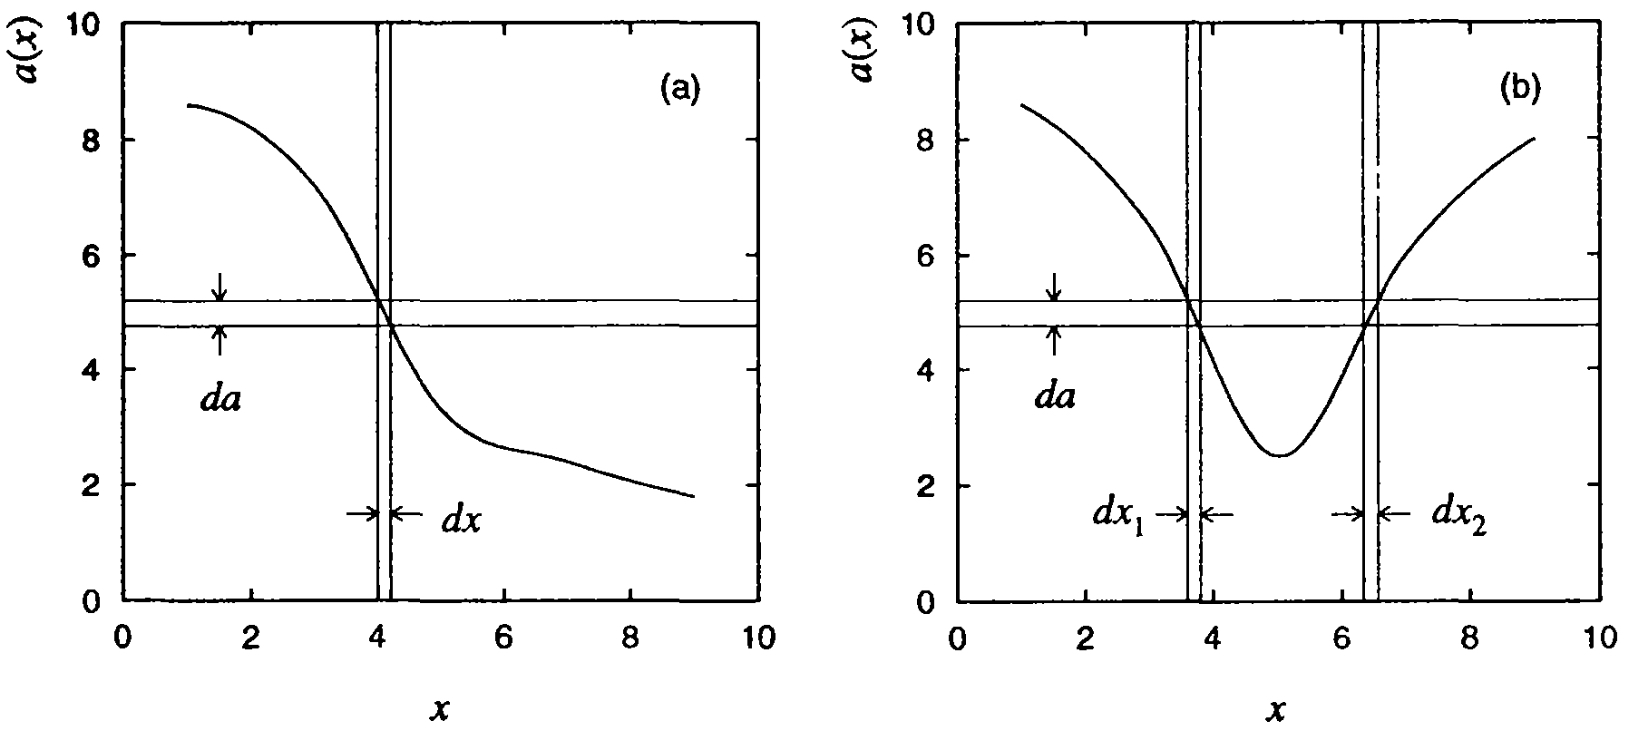
\includegraphics[width=0.65\textwidth,keepaspectratio]{RVfunc}
	\label{fig:RVfunc}
\end{figure}
%Distribuzione di probabilit\'a di $a(X)$ funzione di variabile casuale X con PDF $f(x)$:
\begin{align*}
%&g(a)=f(x(a))|\TDy{a}{x}|\tag*{g(a)\,da=f(x)\,dx}\\
&g(a)\,da=|\int_{x(a)}^{x(a+da)}f(x')\,dx'|=\int_{x(a)}^{x(a)+|\TDy{a}{x}|da}f(x')\,dx'\\
&\Rightarrow g(a)=f(x(a))|\TDy{a}{x}|\\
&g(a')d\,a'=\int_{dS=\{a'\leq a(\vec{x})\leq a'+d\,a'\}}f(x_1,\ldots,x_n)d^n\,x\\
&\prob{(y_1,\ldots,y_n)}=\frac{\prob{(x_1,\ldots,x_n)}}{|\left.\frac{\partial(y_1,\ldots,y_n)}{\partial(x_1,\ldots,x_n)}\right|_{x_1,\ldots,x_n=X_1(\vec{y}),\ldots,X_n(\vec{y})}|}\ (g(\vec{a})=f(\vec{x})|\underset{\PDy{\vec{a}}{\vec{x}}}{J}|)
\end{align*}
\end{frame}

\begin{frame}{Somma di RV: Convoluzione e funzione caratteristica}
\begin{block}{Applicazione cambio di variabile}
Applicando regole cambio variabile per $Z=X+Y$ e $Y'=Y$ e marginalizzando su $Y'$ si trova: $f(Z=X+Y)=\intsinf{}f_X(Z-t)f_Y(t)\,dt$
\end{block}
\begin{block}{Antitrasformata di Fourier prodotto delle funzioni caratteristiche}
\begin{align*}
&X=X_1+X_2\\
&M_X(t)=M_{X_1}M_{X_2}
\end{align*}
La funzione caratteristica determina completamente pdf: se $F(X)$ continua, $dF(X)=f(X)dX$ allora $f(X)=\frac{1}{2\pi}\intsinf{}\phi_X(t)\exp{-iXt}\,dt$.
\end{block}
\end{frame}

\section{Formule propagazione errori}

\begin{frame}{Formule propagazione errori}
\begin{block}{Teorema di Cramer}
$F(X,Y)$ continua,e derivataprima e seconda continua in intorno di $(M_x,M_y)$: RV $W=F(\bar{x},\bar{y})$ is asymptotically normal with $\E{[W]}=F(M_x,M_y)$,
\[\var{[W]}=[\PDy{X}{F}]_M^2\frac{\sigma^2_X}{n}+[\PDy{Y}{F}]_M^2\frac{\sigma^2_Y}{n}+2[\PDy{X}{F}]_M[\PDy{Y}{F}]_M\frac{\sigma_{XY}}{n}\]
\end{block}
\begin{block}{Error propagation}
\begin{align*}
&\E{[\hat{W}]}=\E{[F(\bar{x},\bar{y})]}\\
&=F(M_x,M_y)+\frac{1}{2}\{[\PtwoDy{X}{F}]\frac{\sigma_x^2}{n}+2[\PtwoMDy{X}{Y}{F}]\frac{\sigma_{xy}}{n}+[\PtwoDy{Y}{F}]\frac{\sigma_y^2}{n}\}\\
&\var{\hat{W}}=[\PDy{X}{F}]^2\frac{\sigma_x^2}{n}+[\PDy{Y}{F}]^2\frac{\sigma_y^2}{n}+2[\PDy{X}{F}][\PDy{Y}{F}]\frac{\sigma_{xy}}{n}
\end{align*}
\end{block}
\end{frame}

\begin{frame}{Estimators of population parameters}
\begin{align*}
&\bar{x}=\frac{1}{n}\sum_ix_i&M_x\tag{Mean: first moment}\\
&s_x^2=\frac{1}{n-1}\sum_i(x_i-\bar{x})^2&\sigma_x^2\tag{var: 2nd central moment}\\
&s_{xy}=\frac{1}{n-1}\sum_i(x_i-\bar{x})(y_i-\bar{x})&\sigma_{xy}\tag{covariance}\\
&r_{xy}=\frac{s_{xy}}{s_xs_y}&\rho_{xy}\tag{correlation coefficient}\\
&s_{\bar{x}}=\frac{1}{\sqrt{n}}s_x&\sigma_{\bar{x}}\tag{std deviation of average}\\
&v_x=\frac{s_x}{\bar{x}}&\frac{\sigma_x}{M_x}\tag{relative standard deviation}
\end{align*}
\end{frame}

\section{Funzione caratteristica/generatrice (dei momenti)}

\begin{frame}{Funzione generatrice dei momenti - Funzione caratteristica}
\begin{columns}[T]
	\begin{column}{0.4\textwidth}
		\begin{align*}
		&M_X(t)=\E{[\exp{tX}]}\\
		&\phi_X(t)=\E{[\exp{itX}]}=\int\exp{itx}\,d\mu_X(x)\\
		&\phi(0)=1,\ |\phi(t)|\leq1\\
		&Y=\alpha X+b:\ M_Y=\exp{ibt}M_X(\alpha t)\\
		&\mu_n(x_0)=\E{[\sum_k^n]}\binom{n}{k}(-1)^{n-k}\mu'_kx_0^{n-k}\\
		&E[a(X)]=\intsinf{}a(x)f(x)dx=\intsinf{}ag(a)da
		\end{align*}
%	Non \'e detto che $f(\mu)=\E{[f]}$.
	\end{column}
	\begin{column}{0.6\textwidth}
		\begin{align*}
		&\PDyn{t}{M_X}{n}|_{t=0}=\E{[x^n]}=\mu_n'\\
		&\PDyn{(it)}{\phi_X}{n}|_{t=0}=(-i)^n\E{[x^n]}=\mu_n'\\
		&\phi_X(t)=\E{[\sum_r\frac{(itX)^r}{r!}]}\\
		&=\sum_r\frac{(it)^r}{r!}\E{[X^r]}=\sum_r\frac{(it)^r}{r!}\mu_r'\\
		&\phi_X(t)=1+i\mu t+\frac{1}{2}(\sigma^2+\mu^2)(it)^2
		\end{align*}
	\end{column}
\end{columns}
Determina completamente pdf: se $F(X)$ continua, $dF(X)=f(X)dX$ allora $f(X)=\frac{1}{2\pi}\intsinf{}\phi_X(t)\exp{-iXt}\,dt$
\begin{block}{Levy theorem: if sequenza $\phi_n\to\phi$ allora $X_n\xrightarrow{D}X$}
Per ogni RV con $\mu$ finita $\phi_X(t)\approx1+i\mu t+o(t)$,$\phi_{\frac{1}{n}X}(t)=\phi_X(\frac{t}{n})$, $\phi_{X+Y}(t)=\phi_X(t)\phi_Y(t)$:
$\phi_{\overline{X}_n}(t)=[\phi_X(t)]^n=[1+it\mu+\ldots]^n\to\exp{i\mu t}$
\end{block}
\end{frame}


\begin{frame}{Funzioni caratteristiche}
COwan 157
\end{frame}

\section{Legge grandi Numeri - T limite centrale}

\begin{frame}{Legge grandi numeri}
\begin{itemize}
\item Chebyshev ineq: $\prob{(|X-\mu|\geq k\sigma)}\leq\frac{1}{k^2}$
\item Probability convergence: 	Una sequenza di RV $\{X_n\}\to X$ in probabilit\'a se $\lim_{n\to\infty}\prob{(|X_n-X|)>\epsilon}$=0
\item LLN: $X_1,\ldots,X_n$ iid RV (RV campionata n volte): $\E{X_i}=\mu$, finite variance: $\var{X_i}=\sigma^2$ allora $\prob{(|\overline{X}_n-\mu|>\epsilon)}\leq\frac{\sigma^2}{n\epsilon^2}$, infatti
\begin{align*}
&\var{\overline{X}_n}=\var{\frac{1}{n}(X_1+\ldots+X_n)}\\
&=\frac{1}{n^2}\var{(X_1+\ldots+X_n)}=\frac{n\sigma^2}{n^2}=\frac{\sigma^2}{n}\\
&\prob{(|\overline{X}_n-\mu|>\epsilon)}\leq\frac{\sigma^2}{n\epsilon^2}
\end{align*}
\end{itemize}
\end{frame}

\begin{frame}{LLN: asintoticamente gaussiana - Teorema limite centrale (CLT)}
Se esistono $\mu_1, \mu_2$ finiti vale LLN: $\overline{x}_n-\mu\xrightarrow{P}0$.
\begin{columns}[T]
	\begin{column}{0.5\textwidth}
		\begin{align*}
		&\var{(\overline{x}_n-\mu)}=\var{(\frac{S_N}{N})}\\
		&=\frac{1}{N^2}\var{(S_N)}=\frac{\sigma^2}{N}\\
		&\var{(S_N)}=\sum(\PDy{x_i}{S_N})^2\sigma_i^2
		%&\phi(t)=\phi_{X-\mu}
		\end{align*}
	\end{column}
	\begin{column}{0.5\textwidth}
		\begin{align*}
		&y_N=\sqrt{\frac{N}{\sigma^2}}(\overline{x}-\mu)\\
		&\E{[y_N]}=0,\ \var{[y_N]}=1\\
		&\phi_N=[\phi(\frac{t}{\sigma\sqrt{N}})]^N
		\end{align*}
	\end{column}
\end{columns}
\begin{align*}
&\phi(t)=\sum_{m=0}^{\infty}\left.\frac{d^m\phi}{dt^m}\right|_{t=0}\frac{t^m}{m!}=\sum_{m=0}^{\infty}\frac{(it)^m}{m!}\E{(y^m)}\approx1-\frac{t^2}{2N}\sigma^2-\frac{it^3}{3!}\frac{\E{[(x-\mu)^3]}}{n\expy{3/2}}+\ldots\\
&\log{\phi_N}=N\log{\phi(\frac{t}{\sigma\sqrt{N}})}\approx N[\frac{it\mu}{\sigma\sqrt{N}}+\frac{(it)^2\sigma^2}{2\sigma N}+o(\frac{t^3}{N\expy{\frac{3}{2}}})]\to-\frac{t^2}{2}\\
%\text{Per T Levy la pdf \'e:}\\
&\frac{1}{2\pi}\int\exp{-\frac{t^2}{2}}\exp{-itx}d\,t=\frac{1}{2\pi}\int\exp{(t+ix)^2-\frac{x^2}{2}}d\,t=\frac{1\exp{-\frac{x^2}{2}}}{\sqrt{2\pi}}
\end{align*}
\end{frame}

\begin{frame}{Bernulli, binomiale, Poisson, esponenziale, uniforme (massimo, minimo e mediana), gaussiana}
\todo{Bernulli, binomiale, Poisson, esponenziale, uniforme (massimo, minimo e mediana), gaussiana}
\end{frame}

\begin{frame}{Propriet\'a $\chi^2$}
La distribuzione di chi-squared con $\nu$ gradi di libert\'a $\prob{(\chi_{\nu}^2)}$ \'e la distribuzione di probabilit\'a di $\sum_1^{\nu}x_i^2$ con $x_i\to N(0,1)$ ($\sum_{i=1}^N\frac{(x_i-\mu_i)^2}{\sigma_i^2}$), $\chi^2$ non centrale $x_i\to N(\mu_i,1)$, parametro non centralit\'a $\lambda=\sum\mu_i^2$.
\begin{columns}[T]
	\begin{column}{0.7\textwidth}
		Funzione caratteristica: $y=\frac{(x_i-\mu_i)}{\sigma_i}$, $z=y^2$
		\begin{align*}
		&f(z;n=1)=2\phi(y)|\TDy{z}{y}|=\frac{1}{\sqrt{2\pi z}}\exp{-z/2}\\
		&\phi_1(t)=\E_z{(\exp{itz})}=(1-2it)\expy{-1/2}\\
		%&=\intsinf{}\frac{\exp{itx-x^2/2}}{\sqrt{2\pi}}\,dx=\frac{1}{\sqrt{1-2it}},\\
		&\phi_{\chi^2_{\nu}}(t)=(1-2it)\expy{-\frac{\nu}{2}}
		\end{align*}
	\end{column}
	\begin{column}{0.3\textwidth}
		\begin{align*}
		&\E{(\chi^2_{\nu})}=\nu\\
		&\var{[\chi_{\nu}^2]}=2\nu\\
		&\E{(\chi^{2,NC}_{\nu})}=\nu+\lambda
		\end{align*}
	\end{column}
\end{columns}
\begin{align*}
&\prob{(x=\chi^2_{\nu})}=\frac{1}{2\expy{\nu/2}\Gamma(\frac{\nu}{2})}x\expy{\frac{\nu}{2}-1}\exp{-\frac{x^2}{2}}\xrightarrow{\nu\to\infty}N(\nu,2\nu)
\end{align*}
Approssimazione di Fisher: $\prob{(\sqrt{2\chi^2})}\approx N(\sqrt{2\nu-1},1)$
\end{frame}

\section{Data analysis}

\begin{frame}{Funzione di Likelihood}
\begin{columns}[T]
	\begin{column}{0.5\textwidth}
		$L_{x_0}(m)=p(x_0;m)$, se x,y eventi indipendenti: $L_{(x_0,y_0)}(m)=L_{x_0}(m)L_{y_0}(m)$. Definita a meno di costante moltiplicativa ($\log{L}$): invariante per cambiamento di osservabile (funzione solo dei dati)
		$L_{f(t_0)}(m)=|J(t_0)|L_{t_0}(m)$
	\end{column}
	\begin{column}{0.5\textwidth}
		\begin{block}{T di Bayes e likelihood}
			Prior $p(\theta)$ contiene belief su parametro fino al nostro esperimento:
			\begin{align*}
			&p(\theta|x_0)=\frac{p(x_0|\theta)p(\theta)}{p(x_0)}\\
			&\posterior{}=\frac{\likelihood{}\prior{}}{\int p(x_0|\theta)p(\theta)\,d\theta}
			\end{align*}
			
			Posterior ratio (Degree of belief): $\frac{\Pi(\theta_1|x_0)}{\Pi(\theta_2|x_0)}=\frac{L_{x_0}(\theta_2)}{L_{x_0}(\theta_1)}\frac{\Pi(\theta_2)}{\Pi(\theta_1)}$.
		\end{block}
	\end{column}
\end{columns} 
\begin{columns}[T]
	\begin{column}{0.5\textwidth}
		\begin{block}{Metodo di massima likelihood}
			Ripetendo gli esperimenti la likelihood diventa pi\'u piccata.
		\end{block}
	\end{column}
	\begin{column}{0.5\textwidth}
		
	\end{column}
\end{columns}
\end{frame}

\begin{frame}{Esempi di likelihood}
\begin{columns}[T]
\begin{column}{0.3\textwidth}
	Likelihood per Bernoulli:
	\begin{align*}
	&L_0=1-p\\
	&L_1=p
	\end{align*}
	L per $U(0,m)$:
	\[\frac{1}{m}:\ x<m\]
\end{column}
\begin{column}{0.7\textwidth}
	\begin{block}{N RV iid con pdf esponenziale}
		\begin{align*}
		&\prob{(t,\tau)}=\frac{1}{\tau}\exp{-\frac{t}{\tau}}\\
		&L_{(t_1,\ldots,t_n)}(\tau)=\prod_i^n\frac{1}{\tau}\exp{-\frac{t_i}{\tau}}\\
		&=\frac{1}{\tau^n}\exp{-\frac{\sum t_i}{\tau}}=\frac{1}{\tau^n}\exp{-\frac{n\overline{t}}{\tau}}
		\end{align*}
	\end{block}
\end{column}
\end{columns}
\end{frame}

\begin{frame}{Statistica}
		\begin{block}{Momenti di una statistica S}
	\begin{align*}
	&\E{[(S(\vec{x})-\E{[S]})^l]}
	\end{align*}
\end{block}
\begin{block}{Propagazione errori}
\begin{align*}
&S(\vec{x})\approx y(\vec{\mu})+\left.\sum_i^n\PDy{x_i}{S}\right|_{\vec{\mu}}(x_i-\mu_i)+o(|\vec{x}-\vec{\mu}|)\\
&\var{(S)}=\E{[(S(\vec{x})-\E{[S]})^2]}\approx\sum_{ij}\PDyat{x_i}{S}{\vec{\mu}}\PDyat{x_i}{y}{\vec{\mu}}\cov{x_ix_j}\\
&\cov{x_ix_j}=\E{[(x-\mu_x)(y-\mu_y)]}=\E{[xy]}-\mu_x\mu_y
\end{align*}
\end{block}
\begin{block}{Statistica sufficiente}
Statistica sufficiente $S$ per parametro $\Theta$. Pdf di X data $T(X)$ non dipende da parametro $\theta$: $\prob{(x;S,\theta)}=\prob{(x;S)}$.
Statistica sufficiente minimale
	$S$ sufficiente e esiste una funzione $f$ per ogni $s_i$ con $S=f(s_i)$ e $\dim({S})\leq\dim{(X)}$.
\end{block}
\end{frame}

\begin{frame}{Statistiche sufficienti per il parametro dato. T di Darmois}
\begin{block}{Teorema di fattorizzazione}
	Probabilit\'a di osservare $X$ dato $\theta$ \'e probabilit\'a di $S(x)$ dato $\theta$ per funzione sole osservabili: $\prob{(x;\theta)}=\prob{(S(x);\theta)}h(x)$ e $\omega_{\theta}$ non dipende da $\theta$
\end{block}
\begin{block}{Teorema di Darmois: condizione necessaria e sufficiente per esistenza statistica sufficiente}
	Esiste S tale che $\dim{(S)}<\dim{(X)}$ iff
	\begin{align*}
	&p(\vec{x}|\theta)=\Exp{[\sum_i^n\alpha_i(\vec{x})a_i(\theta)+\beta(\vec{x})+\gamma(\theta)}\\
	&S_j=\sum_i\alpha_j(x_i)
	\end{align*}
	Esiste statistica suff. iff: supporto pdf non dipende da parametro e appartiene alla famiglia esponenziale.
\end{block}
\end{frame}

\begin{wordonframe}{Dimostrazioni S sufficiente}
\begin{block}{n RV iid con pdf bernoulli p}
	$X_1,\ldots,X_n$: iid con pdf di Bernoulli, supporto pdf $\chi=\{0,1\}$, parametro p nell'intervallo $(0,1)$:
	\begin{align*}
	&T=\sum X_i\to\{0,\ldots,n\}&\intu{con pdf binomiale}
	&\prob{(X_1=x_1\cap\ldots X_n=x_n|T=t)}=0, t\neq\sum x_i\\
	&=\prob{(\cap_iX_i=x_i|T=t)}=\frac{\prob{((\cap_iX_i=x_i)\cap(T=t))}}{\prob{(T=t)}}=\frac{\prob{(\cap_iX_i=x_i)}}{\prob{(T=t)}}\intu{se $\sum x_i=t$:}
	&A=\{\cap_iX_i=x_i\}\subseteq B=\{T=t\}
	\end{align*}
	e poich\'e le $X_i$ sono indipendenti si ha
	\begin{align*}
	&\frac{\prod\prob{(X_i=x_i)}}{\prob{(T=t)}}=\frac{p^{\sum x_i}(1-p)^{n-\sum x_i}}{\binom{n}{t}p^t(1-p)^{n-t}}
	\end{align*}
\end{block}
\begin{block}{n RV iid Poisson$(\lambda)$}
	$X_1,\ldots,X_n$: iid con pdf di Poisson con parametro ignoto $\lambda$:
	\begin{align*}
	&\prob{(X_1=x_1\cap\ldots X_n=x_n|T=t)}=\prob{(\cap_iX_i=x_i|T=t)}\\
	&\frac{\prob{((\cap_iX_i=x_i)\cap(T=t))}}{\prob{(T=t)}}=\frac{\prob{(\cap_iX_i=x_i)}}{\prob{(T=t)}},\ t=\sum x_i\\
	&=\frac{\prod_i[\frac{\exp{-\lambda}\lambda^{x_i}}{x_i!}]}{\frac{\exp{-\lambda}(n\lambda)^t}{t!}}=\frac{t!}{\prod x_i!}n^{-t}
	\end{align*}
\end{block}
\begin{block}{Gaussiana: media ignota, varianza nota}
	\begin{align*}
	&L(\overline{x};\mu)=\prod_iL(x_i;\mu,\sigma)=(\frac{1}{\sqrt{2\pi}\sigma})^N\underbrace{\exp{-\frac{N}{2}\frac{\sum_i(\overline{x}-\mu)^2}{\sigma^2}}}_{g(T,\theta)}\underbrace{\exp{-\frac{N}{2}\frac{\sum_i(x_i-\overline{x})^2}{\sigma^2}}}_{h(\vec{x})}
	\end{align*}
	La statistica ''media aritmetica'' \'e sufficiente per parametro $\mu$ della gaussiana (dominio gaussiana non dipende da $\mu$) (Ex: pdf della media aritmetica)
\end{block}
\begin{block}{Gaussiana: media nota, varianza ignota}
	$\hat{\sigma}^2=\frac{\sum x_i^2-\mu}{N}$ \'e sufficiente per $\sigma^2$ (pdf di $\hat{\sigma}^2\propto g$ e dominio gaussiana non dipende da $\sigma$). (Ex: statistica sufficiente $\sigma$ gaussiana)
\end{block}
\begin{block}{Media aritmetica \'e statistica sufficiente per parametro binomiale, poissoniana, esponenziale}
	\begin{align*}
	&\prob{(k)}=\binom{n}{k}p^k(1-p)^{n-k}\\
	&\prob{(k)}=\frac{\mu^k\exp{-\mu}}{k!}\\
	&\prob{(x)}=\lambda\exp{-\lambda x}
	\end{align*}
\end{block}
\begin{block}{Distribuzione uniforme: $x_{max}$ statistica sufficiente.}
	\begin{columns}[T]
		\begin{column}{0.5\textwidth}
			\pgfmathsetmacro{\unifM}{3}
			\begin{tikzpicture}[scale=0.5,domain=0:1.5*\unifM]
			\pgfmathsetmacro{\unifN}{(\unifM)^-1}
			\begin{axis}[ylabel={$p(x;m)$},extra x ticks={\unifM}, extra x tick labels={$m$},
			extra x tick style={xticklabel style={yshift=-10}}]
			%\draw[->] (-0.2,0) -- (1.5*\unifM,0) node[right] {$x$};
			%\draw[->] (0,-0.2) -- (0,1.5*\unifM) node[above,red] {$p(x;m)$};
			%\draw[color=red] plot[domain=0:\unifM, id=unif] function{\unifN} node[right] {$\frac{1}{m}$};
			\addplot[color=red] function [raw gnuplot, id=unifpdf, mark=none]{set xrange [0:\unifM]; plot \unifN};
			\end{axis}
			\end{tikzpicture}
		\end{column}
		\begin{column}{0.5\textwidth}
			\begin{align*}
			&\prob{(x;m)}=\left\{\begin{matrix}\frac{1}{m}\ x\in[0,m]\\0\\\end{matrix}\right.&\intertext{estraggo N $x_1,\ldots,x_n$}\\
			&L(\vec{x},m)=\prod_iL(x_i;m)=\left\{\begin{matrix}\frac{1}{m^N}\ m>x_{max}\\0\ m<x_{max}\\\end{matrix}\right.
			\end{align*}
		\end{column}
	\end{columns}
	%$g(T,\theta)\propto A(T;\theta)$ dove $A$ \'e pdf di statistica $T$?
	\begin{align*}
	&\prob{(x_{max}<x_0)}=F_M(x_0)=\prod_i\prob{(x_i<x_0)}=\prod_i\int_0^{x_0}\frac{1}{m}\,dx=(\frac{x_0}{m})^N\\
	&\prob{(x_M;m)}=\TDof{x_0}\left.F_M(x_0)\right|_{x_M}=\frac{N}{m}(\frac{x_M}{m})^{N-1}I(x_M<m)\\
	&L_{\vec{x}}(m)=\frac{N}{m^N}x_M^{N-1}\frac{1}{Nx_M^{N-1}}=\prob{(x_M;m)}\frac{1}{Nx_M^{N-1}}\ m>x_M
	\end{align*}
	$\prob{(x;S,\theta)}=\prob{x;S}$!
\end{block}
\end{wordonframe}

\section{Informazione}

\begin{frame}{Informazione di Fischer}
Informazione contenuta nei dati su un parametro $\Theta$
\begin{align*}
&\overbrace{I_X(\Theta)}^{\text{n RV iid:}=nI_{X_1}}=\E_{\Theta}{[(\PDof{\Theta}\log{f(X;\Theta}))^2]}=\overbrace{-\E_{\Theta}{[\PtwoDof{\Theta}\log{f(X;\Theta)}]}}^{\text{se esistono finiti $\PtwoDof{\Theta}$ e $\E{}$}}
\end{align*}
Per due parametri:
\begin{align*}
&I_X(\Theta)=\begin{pmatrix}I_{11}(\Theta)&I_{12}(\Theta)\\I_{21}(\Theta)&I_{22}(\Theta)\end{pmatrix}\ I_{ij}(\Theta)=-\E{[\frac{\partial^2}{\partial\Theta_i\partial\Theta_j}\log{f(X;\Theta)}]}
\end{align*}
\begin{block}{Score statistics}
	\begin{columns}[T]\begin{column}{0.5\textwidth}
			
		\end{column}\begin{column}{0.5\textwidth}
		$I_X(\Theta)\geq I_T(\Theta)$: l'uguaglianza vale iff T \'e sufficiente per $\Theta$.
	\end{column}\end{columns}
\end{block}
\end{frame}

\begin{wordonframe}{Esempi Informazione}
\begin{columns}[T]
\begin{column}{0.5\textwidth}
	\begin{block}{pdf Poisson}
		\begin{align*}
		&\log{f}=-\lambda+x\log{\lambda}-\log{x!}\\
		&I_X(\lambda)=\invers{\lambda}
		\end{align*}
	\end{block}
\end{column}
\begin{column}{0.5\textwidth}
	\begin{block}{pdf Gauss}
		\begin{align*}
		&\log{f}=-\frac{1}{2}\frac{(x-\mu)^2}{\sigma^2}-\log{(\sqrt{2\pi}\sigma)}\\
		&I_X(\mu)=\sigma\expy{-2}
		\end{align*}
	\end{block}
\end{column}
\end{columns}
\begin{block}{n RV iid}
\begin{columns}[T]
	\begin{column}{0.5\textwidth}
		$X_1,\ldots,X_n$ n RV iid:
		\begin{align*}
		&X=\sum X_i\\
		&I_X(\Theta)=nI_{X_1}(\Theta)
		\end{align*}
	\end{column}
	\begin{column}{0.5\textwidth}
		proof pg 327 probability and statistical inference
	\end{column}
\end{columns}
\end{block}
\begin{block}{n RV gaussiane $N(\mu,\sigma^2)$: matrice informazione}
$\vec{X}=(X_1,\ldots,X_n)$ e $\vec{\Theta}=(\mu,\sigma^2)$
\begin{align*}
&I_{11}=\E{[(\PDof{\mu}\log{f})^2]}=\sigma\expy{-2}\ I_{22}=\E{[(\PDof{\sigma^2}\log{f})^2]}=\frac{1}{2}\sigma\expy{-4}\\
&I_{12}=I_{21}=\frac{1}{2\sigma^2}\E{[\sigma\expy{-3}(X_1-\mu)^3-(X_1-\mu)]}=0
\end{align*}
\end{block}
\begin{block}{Statistica $x_m$ non \'e consistente}
\begin{align*}
&\E{[x_m]}=\int\,dx_mx_mf(x_m;m)=\int\,dx_mx_m\frac{N}{m}[1-\frac{x_m}{m}]^{N-1}=\frac{m}{N+1}\\
&\E{[x_m^2]}=\int\,dx_mx_m^2f(x_m;m)=\int\,dx_mx_m^2\frac{N}{m}[1-\frac{x_m}{m}]^{N-1}\\
&=\frac{2m^2}{(N+1)(N+2)}\\
&\var{[x_m]}=\E{[x_m^2]}-\E^2{[x_m]}=\frac{N}{(N+1)^2(N+2)}m^2\to0\\
&\hat{m}=(N+1)x_m:\ \E{[\hat{m}]}=m,\ \var{[\hat{m}]}=\frac{N^2}{(N+1)(N+2)}m^2\\
&I_{x_m}(m)=\frac{N}{(N-2)m^2},\ (CR:\ \frac{N}{N+2}\geq\frac{N-2}{N})
\end{align*}
$\hat{m}$ non \'e consistente: non converge in probabilit\'a al parametro.
\end{block}
\end{wordonframe}

\section{Stima puntuale}

\begin{frame}{Propriet\'a generali stiamatori}
Statistica $\hat{\Theta}(X_1,\ldots,X_n)$ che fornisce stima di funzione dei parametri $\tau(\Theta)$
\begin{itemize}
	\item Consistenza (LGN): $\prob{\hat{\theta}}\to\theta_0$
	\item Varianza $\var{\vec{X}}\to\frac{1}{N}$ - Bias $b(\vec{x})$ non diminuisce all'aumentare delle misure; scuola soggettivista: bias non esiste.
	\item distribuzione semplice
\end{itemize}
\begin{columns}[T]
	\begin{column}{0.45\textwidth}
	Riduzione del bias:
		\begin{align*}
	&\E{[S(x)]}=\theta+b(\theta)\\
	&\to\ S'(x)=S(x)-b(\hat{\theta})-\hat{b}(x)\\
	&\E{[\hat{b}(x)]}=b(\hat{\theta})\\
	&\var{[S']}=\var{[S]}+\var{[b]}
	\end{align*}
	Metodo empirico
	\begin{align*}
	&S_N'(x)=2S_N(x)\\
	&-\frac{1}{2}[S_{\frac{N}{2}}(x_1,\ldots,x_{\frac{N}{2}})+S_{\frac{N}{2}}(x_{\frac{N}{2}},\ldots,x_N)]
	\end{align*}
	\end{column}
	\begin{column}{0.55\textwidth}
		\begin{itemize}
			\item unbiased estimator: $\E_{\Theta}[T]=\tau(\Theta)$
			\item estimator bias: $B_{\Theta}(T)=\E_{\Theta}[T]-\tau(\Theta)$
			\item Estimator mean square error: $\E{[(T-\tau(\Theta))^2]}=V_{\Theta}[T]+(\E{[T]}-\tau(\Theta))^2$
			\item Stimatori consistenti: $\lim_{n\to\infty}T_n(X_1,\ldots,X_n)\overset{P}{=}\tau(\Theta)$
		\end{itemize}
	\end{column}
\end{columns}
\end{frame}

\begin{frame}{Best unbiased estimator: Disuguaglianza di Cramer-Rao (CRLB)}
$X_1,\ldots,X_n$ iid con pdf $f(x,\Theta)$: se supporto $\Omega_{\Theta}$ di $f(x,\Theta)$ non dipende da $\Theta$ e integrali in $dx$ sono invertibili con $\PDof{\Theta}$; esiste stimatore unbiased $T(\vec{X})\xrightarrow{\E{[\ ]}}\tau(\Theta)$ con $\PDy{\Theta}{\tau}$ esiste finito, allora:
\begin{align*}
&V_{\Theta}[T]\geq\frac{[\tau'(\Theta)]^2}{n\E_{\Theta}[(\PDof{\Theta}\log{f(X_1;\Theta)})^2]}=\frac{[\tau'(\Theta)]^2}{nI_{X_1}(\Theta)}\\
&\left(\frac{(1+\TDy{\theta}{b})^2}{I_{\hat{\Theta}}(\theta)}\right)
\end{align*}
minimum variance bound
\end{frame}

\section{Costruzione stimatori consistenti}

\begin{frame}{Logica stimatori consistenti - Stimatori impliciti}
Consistenza: $\hat{\theta}\xrightarrow{P}\theta_0$. Una quantit\'a con queste caratteristiche \'e
\[\xi=\invers{N}\sum_ia(X_i)\xrightarrow{N\to\infty}\E{[a(X)]}=\int a(X)f(X;\theta)\,dX=h(\theta)\]
dove $a(X)$ \'e qualsiasi funzione di X con varianza finita: per LLN sample mean is C-estimator of $a(X)$. We find $a(X,\theta)$ in maniera che $h(\theta_0)=0$ per il valore vero di $\theta_0$, $\xi(\hat{\theta})=0$, stimatore implicito:
\begin{align*}
&\xi(\theta)=\frac{1}{N}\sum_ia(X_i,\theta),\ \xi(\theta_0)\xrightarrow{N\to\infty}\E{[a(X,\theta_0)]}=0
\end{align*}
One of the root of $h(\theta)$ give consistent estimate of $\theta_0$ if $\xi$ is differentiable, mean of $\xi$, $\PDy{\theta}{\xi}$ exist and $\lim_{N\to\infty}\E{[\PDy{\theta}{\xi(\theta)}]_{\theta=\theta_0}}\neq0$
Moment method:
\begin{align*}
&a(X_i,\theta)\to a(X_i,\theta)-\E{[a(X)]}\\
&g(X_i,\theta)=a(X_i)\theta-\int_{\theta_0}^{\theta}\int a(X)f(X,\theta)\,dX\,d\theta
\end{align*}
in practice one find $a(X_i,\theta)$ minimizing other function g: $a(X_i,\theta)=\PDof{\theta}g(X_i,\theta)$ - maximum likelihood and minimum $\chi^2$
\end{frame}

\begin{frame}{Momenti}
Ho N osservazioni $x_1,\ldots,x_n$ di RV iid con pdf $f(x,\theta)$, $\theta=(\theta_1,\ldots,\theta_m)$. Cerco m funzioni linindip $a_i(X)$ quindi il valore di aspettazione dipende dal valore vero del parametro:
\[\E{[a_i(x)]}=\int a_i(x)f(x;\theta)\,dx=e_i(\theta)\to\E{[m_k]}=\frac{\sum_i\E{[x_i^k]}}{N}=\mu'_k\]
convergono in probabilit\'a ai momenti della distribuzione.
\begin{columns}[T]
\begin{column}{0.65\textwidth}
	\begin{align*}
	&\cov{(m_i,m_j)}=\E{[m_im_j]-\E{[m_i]}\E{[m_j]}}\\
	&=\frac{\mu'_{i+j}-\mu_i'\mu_j'}{N}\\
	&\cov{[\hat{\theta}_i,\hat{\theta}_j]}=\sum_{k,l}\PDy{\hat{e}_k}{\hat{\theta}_i}\PDy{\hat{e}_l}{\hat{\theta}_j}\cov{[\hat{e}_k,\hat{e}_l]}
	\end{align*}
	Co-var matrix of estimators (error propagation formula)
\end{column}
\begin{column}{0.35\textwidth}
	\begin{align*}
	&m_1=\mu_1'(\theta_1,\ldots,\theta_n)\\
	&\vdots\\
	&m_n=\mu_n'(\theta_1,\ldots,\theta_n)\intd{Invertendo il sistema sopra si trovano gli stimatori:}
	&\hat{\theta_1}(m_1,\ldots,m_m)\\
	&\vdots\\
	&\hat{\theta_m}(m_1,\ldots,m_m)
	\end{align*}
\end{column}
\end{columns}
\end{frame}

\begin{wordonframe}{Examples moment estimators}
\begin{columns}[T]\begin{column}{0.5\textwidth}
	\begin{block}{Uniforme $U(a,b)$}
		\begin{align*}
		&\mu_1=\E{[X]}=\frac{1}{2}(a+b)\\
		&\mu_2=\E{[X^2]}=\frac{1}{3}(a^2+ab+b^2)\\
		&\hat{a}=\mu_1\pm\sqrt{3(\mu_2-\mu_1^2)}\\
		&\hat{b}=2\mu_1-a
		\end{align*}
	\end{block}
\end{column}\begin{column}{0.5\textwidth}
	
\end{column}\end{columns}
\end{wordonframe}

\begin{frame}{Stimatori di massima likelihood: derivazione tramite stimatori impliciti}
\begin{align*}
&a(X,\theta)=\PDy{\theta}{\log{L}}=\PDof{\theta}g(X_i,\theta)\\ &K_N=\xi=\frac{1}{N}\PDof{\theta}\sum_i^Ng(X_i,\theta)=\frac{1}{N}\sum_i\PDy{\theta}{\log{(L(x_i,\theta))}}=0\\
&\PDof{\theta}\sum_i^N\ln{f(X_i,\theta)}=\PDof{\theta}\ln{L(\vec{X},\theta)}=0 \tag*{(Likelihood equation)}\\
&K_N=\frac{1}{N}\PDof{\theta}\sum_i^Ng(X_i,\theta)=0: \E{[\PDy{\theta}{\xi}|_{\theta_0}]}=\E{[\frac{1}{N}\PtwoDy{\theta}{\ln{L(\vec{X},\theta)}}|_{\theta_0}]}\\
&\E{[\PDy{\theta}{\xi}|_{\theta_0}]}\xrightarrow{N\to\infty}\E{[\PtwoDy{\theta}{\ln{f(X,\theta)}}|_{\theta_0}]}\\
&\E{[\PDy{\theta}{K}]}=\E{[\PtwoDy{\theta}{\log{L}}]}=-\E{[(\PDy{\theta}{\ln{f(X,\theta)}})^2]}=-I_X<0
\end{align*}
The quantity $\PDof{\theta}\ln{L(\vec{X},\theta)}$ \'e asintoticamente gaussiano con media 0 e varianza $NI(\theta)$
\end{frame}

\begin{frame}[allowframebreaks]{Propriet\'a MLE}
\begin{block}{Consistente se soluzione della likelihood equation \'e unica: massimo assoluto (asintotico) \'e consistente}
$\PDy{\theta}{\log{L_{tot}}}=0$.
\end{block}
\begin{block}{Invariante per trasformazione di parametro}
\end{block}
\begin{block}{Asintoticamente un-biased}
\end{block}
\begin{block}{Asintoticamente efficente: $\var{[\hat{\theta}]}\to\frac{1}{NI_{X_1}}$}
\begin{align*}
&K_N(\hat{\theta)}=K(\theta_0)+\PDy{\theta}{K_N}(\hat{\theta}-\theta_0)+o(\hat{\theta}-\theta_0)^2\intd{prendendo il valore di aspettazione}
&0=\sum_i\frac{\PDy{\theta}{\log{(L(x_i))}}}{N}-I(\hat{\theta}-\theta_0)+(\var{[\hat{\theta}]})\\
&\hat{\theta}-\theta_0\propto N(0,\frac{1}{NI})+\frac{\const{}}{N}: \lim_{N\to\infty}b(\hat{\theta})\propto\frac{1}{N}
\end{align*}
\end{block}
\begin{block}{Pdf dello stimatore tende asintoticamente ad gaussiana}
\end{block}
\begin{block}{MLE per pdf esponenziale}
Per pdf esponenziale\[f(x;\theta)=\exp{\alpha(x)a(\theta)+\beta(x)+c(\theta)}\] il metodo di massima likelihood determina lo stimatore efficiente e senza bias $\hat{M}=\frac{1}{N}\sum_i\alpha(x_i)$ di $M(\theta)=-\frac{\TDy{\theta}{c(\theta)}}{\TDy{\theta}{a(\theta)}}$.
\end{block}
\end{frame}

\begin{wordonframe}{MLE in pratica}
\begin{block}{binning}
\begin{columns}[T]
\begin{column}{0.5\textwidth}
N fissato
\begin{align*}
&\prob{(\vec{k},\theta)}=\frac{N!}{\prod_ik_i!}\prod_i{\underbrace{\prob{(i)}}_{\int_{S_i}\prob{(x|\theta)}\,dx}}\mkern-20mu^{k_i}\\
&\max{[\sum_i k_i\log{[\prob{(x;\theta)}\Delta]}]}\\
&\to\max{[\sum_i \log{[\prob{(n_i;\theta)}]}]}
\end{align*}
\end{column}
\begin{column}{0.5\textwidth}
N variabile: Extended likelihood, normalizzazione varia
\begin{align*}
&\mu_i=\mu_TP_i(\theta)\\
&\prob{(k_i\theta)}=\frac{\prod_i\exp{-\mu_TP_i}(\mu_TP_i)^{k_i}}{k_i!}\\
&\log{L}=\sum_ik_i\log{P_i(\theta)}+k_i\log{\mu_T}\\
&-\mu_TP_i-\bcancel{\log{k!}}\\
&\left\{\begin{matrix}\mkern-240mu\PDy{\theta_i}{\log{L}}=0\\\PDy{\mu_T}{\log{L}}=0\ (:L(\bcancel{\mu_T}),\mu_T(\bcancel{\theta_i}) \Rightarrow\ \mu_T=N)\\\end{matrix}\right.
\end{align*}
\end{column}
\end{columns}
\end{block}

\begin{block}{Fit resolution of histogram (??)}
$A=\sum_i\frac{1}{P_i}(\PDy{\theta}{P_i})^2$
\end{block}\end{wordonframe}

\begin{wordonframe}{Esempi di stimatori di massima likelihood}
Binomiale: $K_1,\ldots,K_N:\ f(k;n,p)=\binom{n}{p}p^k(1-p)^{n-k}$
\begin{align*}
&\log{(L(\vec{k},p))}=\log{[\prod_i^N\binom{n}{k_i}p^{k_i}(1-p)^{n-k_i}]}\\
&\max{(L)}:\ \TDof{p}\log{(L)}=\sum_i^N[\frac{k_i}{p}+(n-k_i)\frac{(-1)}{1-p}]=0\Rightarrow\sum^Nk_i=Nnp\\
&\hat{p}_{MLE}=\sum\frac{k_i}{Nn}=\exv{k}\\
&\E{[\hat{p}]}=\frac{1}{N}\frac{\sum\E{[k_i]}}{n}=\frac{\sum^Npn}{nN}=p\\
&\var{[\hat{p}]}=\var{[\frac{1}{nN}\sum k_i]}=\frac{1}{n^2N^2}Nnp(1-p)\\
&I_{k_i}(p)=\frac{nN}{p(1-p)}\to\frac{1}{\var{}}: MVB
\end{align*}
Gaussiana
Ho N misure $x_i$ da RV con distro gaussiana: cerco MLE per $\mu, \sigma^2$.
\begin{columns}[T]
\begin{column}{0.5\textwidth}
\begin{align*}
&G(x;\mu,\sigma)=\frac{1}{\sqrt{2\pi\sigma^2}}\exp{-\frac{(x-\mu)^2}{2\sigma^2}}\\
&\log{L}=-N\log{\sigma}-\frac{1}{2\sigma^2}\sum_i^N(x_i-\mu)^2\\
&\E{[\hat{\sigma^2}]}=\frac{1}{N}\sum_i\E{[x_i^2-2x_i\exv{x}+\exv{x}^2]}\\
&\E{[x_i^2]}=\mu^2+\sigma^2\\
&\E{[x_i\exv{x}]}=\frac{1}{N}\E{[x_i^2+\sum_{j\neq i}x_ix_j]}\\
&\E{[\exv{x}^2]}=\E{\frac{\sum x_i\sum x_j}{N^2}}=\mu^2+\frac{\sigma^2}{N}
\end{align*}
\end{column}
\begin{column}{0.5\textwidth}
Maximum of $\log{L}$ for $\mu, \sigma^2$
\begin{align*}
&\PDy{\mu}{\log{L}}=0\\
&\hat{\mu}=\frac{\sum x_i}{N}\\
&\PDy{\sigma}{\log{L}}=0\\
&-\frac{N}{\sigma^2}+\frac{1}{\sigma^4}\sum^N(x_i-\exv{x}(\to\mu))=0\\
&\hat{\sigma^2}=\frac{\sum(x_i-\exv{x})^2}{N}\intd{T darmois in 2D: stat. suff.:}
&\sum x_i,\ \sum x_i^2
\end{align*}
\end{column}
\end{columns}
$\E{[\hat{\sigma^2}]}=\frac{N-1}{N}\sigma^2$ quindi definisco lo stimatore unbiassato $\hat{\sigma^2}'=\frac{\sum(x_i-\exv{x})^2}{N-1}$.

\begin{columns}[T]
\begin{column}{0.6\textwidth}
Esponenziale: cambio di parametro. $p(x;\tau)=\frac{1}{\tau}\exp{-\frac{x}{\tau}}=\lambda\exp{-\lambda x}=p(x;\lambda)$:
\end{column}
\begin{column}{0.4\textwidth}
likelihood \'e invariante per cambio di parametro
\end{column}
\end{columns}
\begin{columns}[b]
\begin{column}{0.4\textwidth}
$\hat{\tau}_{MLE}=\frac{\sum_ix_i}{N}:\ \E{[\hat{\tau}]}=\tau,\ I_x(\tau)=\frac{1}{\var{\hat{\tau}}},\ \var{\hat{\tau}}=\frac{\tau^2}{N}$
\end{column}
\begin{column}{0.6\textwidth}
$\log{L}=N\log{\lambda}-\lambda\sum_ix_i$, $\TDy{\lambda}{\log{\lambda}}=0$. $\hat{\lambda}=\frac{N}{\sum x_i}=\frac{1}{\hat{\tau}}$, $\E{[\hat{\lambda}]}=\frac{N}{N-1}\lambda$
\end{column}
\end{columns}
\begin{align*}
&\phi_x(k)=\E{[\exp{ikx}]}=\intzi\exp{ikx}\exp{-\lambda x}\lambda\,dx=\frac{1}{1-i\frac{k}{\lambda}}\\
&\phi_{\sum x_i}\frac{1}{(1-\frac{ik}{\lambda})^N},\ z=\sum x_i\ \text{distribuzione di Erlang}\downarrow\\
&\prob{(z)}=\frac{1}{2\pi}\intsinf{}\frac{\exp{-ikz}}{(1-\frac{ik}{\lambda})^N}\,dk=\frac{\lambda^N}{(N-1)!}z^{N-1}\exp{-\lambda z}
\end{align*}
\begin{columns}[T]
\begin{column}{0.65\textwidth}
\begin{align*}
&\var{[\hat{\lambda}]}=\frac{N^2}{(N-1)^2(N-2)}\lambda^2\to\frac{\lambda^2}{N}\\
&M(\lambda)=-\frac{\TDy{\lambda}{c(\lambda)}}{\TDy{\lambda}{a(\lambda)}}=-\frac{\frac{1}{\lambda}}{-1}=\frac{1}{\lambda}
\end{align*}
\end{column}
\begin{column}{0.35\textwidth}
\begin{align*}
&\alpha(x)=x\\
&a(\lambda)=\lambda\\
&\beta(x)=0\\
&c(\lambda)=\log{\lambda}
\end{align*}
\end{column}
\end{columns}
Ex: pdf di $\frac{1}{\sum x_i}$: funzione caratteristica o ''convoluzione''
Ex: Cambiamento di variabile pdf Erlang
\begin{align*}
&z\to\frac{z}{N}=\exv{x}=\hat{\tau}\\
&\exv{x}\to\frac{1}{\exv{x}}=\hat{\lambda}
\end{align*}
Ex: MLE per $x_{max}$ e $x_{min}$ per pdf uniforme
Per $x_{min}$: \[p(x_{min},m)=\frac{N}{m}[1-\frac{x_{min}}{m}]^{N-1}\] con $x_{min}\in[0,m]$,
\begin{align*}
&\log{L}=\log{N}-\log{m}+(N-1)\log{(1-\frac{x_{min}}{m})}\\
&\TDy{m}{\log{L}}=-\frac{1}{m}+(N-1)\frac{1}{1-\frac{x_{min}}{m}}(\frac{-1}{m^2})=0\\
&\hat{m}_{MLE}=Nx_{min}:\ \E{[\hat{m}]}=\frac{N}{N+1}m,\ \var{\hat{m}}=\frac{N^3}{(N+1)^2(N+2)}m^2
\end{align*}
lo stimatore non \'e consistente.
MLE per poissoniana
\begin{align*}
&P(k;\mu)=\frac{\mu^k\exp{-\mu}}{k!}\\
&
\end{align*}
\end{wordonframe}

\begin{frame}{Massima likelihood e metodo minimi quadrati}
%Se i conteggi (binned case) sono distribuiti in maniera normale attorno al valore $\mu_TP_i$ la minimizzazione del $\chi^2$ \'e equivalente alla massimizzazione della likelihood
N gaussiane iid con media $\mu$ ($\mu_TP_i$ nel caso Poissoniano: $P_=\prob{k_i}$) ignota e varianza $\sigma_i$ nota
\begin{align*}
&\prob{(k_i,\theta)}\propto\exp{-\frac{(k_i-\mu_i)^2}{2\sigma_i^2}}\intd{$\log{L}$ \'e massimizzato dalla funzione che minimizza}
&\chi^2=-2\log{L}=\sum_i^N\frac{(y_i-\mu(x_i;\theta_1,\ldots,\theta_m))^2}{\sigma_i^2}(=\sum_i\frac{(k_i-\mu_i(\theta))^2}{\sigma_i^2})\intd{if measures are not indipendent}
&\log{(L(\theta))}=-\frac{1}{2}\sum_{ij}(y_i-\mu_i(\theta))[\invers{V}]_{ij}(y_j-\mu_j(\theta))
\end{align*}
I parametri che minimizzano $\chi^2$ are LS estimators  $\hat{\theta}_1,\ldots,\hat{\theta}_m$. Binned data:
\begin{align*}
&\chi^2(\theta)=\sum_i^N\frac{(y_i-\lambda_i(\theta)^2)}{\sigma_i^2}\xrightarrow{n\gg np_i}\sum_i^N\frac{(y_i-\lambda_i(\theta))^2}{\lambda_i(\theta)}=\sum_i^N\frac{(y_i-np_i(\theta))^2}{np_i(\theta)}\\
&\lambda_i=\E{[y_i]}=n\int_{x_{min}^i}^{x_{max}^i}=np_i(\theta)\tag{number of entries in bin i}
\end{align*}
\end{frame}

\begin{frame}{Best linear unbiased estimator. Teorema di Gauss-Markov}
se la dipendenza della media ignota dai parametri \'e lineare
\[\lambda_i(\theta)=\mu_i(\theta)=\sum_ja_j(\vec{x})\theta_j=\sum_j^mA_{ij}\theta_j\]
$a_j(\vec{x})$ lin. indip., allora $\hat{\theta}_j$ sono unbiased e al MVB: teorema di Gauss-Markov.
Per dati da gaussiana multi-dimensionale con $\vec{\mu}$ ignota ma covarianza $V$ nota
\begin{align*}
&\chi^2=(\vec{y}-\vec{\lambda})^T\invers{V}(\vec{y}-\vec{\lambda})=(\vec{y}-A\vec{\theta})^T\invers{V}(\vec{y}-A\vec{\theta})\\
&\nabla\chi^2=-2(A^T\invers{V}\vec{y}-A^T\invers{V}A\vec{\theta})=0\tag*{condizione di minimo}\\
&\hat{\vec{\theta}}=\invers{(A^T\invers{V}A)}A^T\invers{V}\vec{y}=B\vec{y}\intd{e matrice di covarianza:}
&U=BVB^T=\invers{(A^TVA)}=\cov{(\theta_i,\theta_j)},\ [\invers{U}]_{ij}=\frac{1}{2}\left[\frac{\partial^2\chi^2}{\partial\theta_i\partial\theta_j}\right]|_{\theta=\hat{\theta}}
\end{align*}
above coincides with CR-bound for inverse covariance matrix when $y_i$ are Gaussian distributed ($\log(L)=-\chi^2/2$)
\end{frame}

\begin{frame}{Esempi di LS estimators}
\begin{itemize}
\item Combine many measures $y_i$ of $\lambda$ with estimated error $\sigma_i$: $\hat{\lambda}=\frac{\sum_iy_i/\sigma_i^2}{\sum_i1/\sigma_i^2}$, $\var[\hat{\lambda}]=\frac{1}{\sum\frac{1}{\sigma_i^2}}$; for not independent measures:
\begin{align*}
&\chi^2(\lambda)=\sum_{i,j}(y_i-\lambda)(\invers{V})_{i,j}(y_j-\lambda)\\
&w_i=\frac{\sum_j(\invers{V})_{ij}}{\sum_{k,l=1}\invers{V}_{kl}},\ \hat{\lambda}=\sum_iw_iy_i\\
&\var{[\hat{\lambda}]}=\sum_{i,j}w_iV_{ij}w_j
\end{align*}
\end{itemize}
\end{frame}

\section{Stima intervallare}

\begin{frame}[fragile]{Bayesian credibility Interval}
\begin{block}{Credibility (della posterior)}
	\begin{align*}
	&\cred{(x)}=\int_{\mu\in\inf(x)}\Pi(\mu|x)\,d\mu=\int_{\mu\inf(x)}\frac{\prob{(x|\mu)}\prob{(\mu)}}{\int\,d\mu}\,d\mu>\cl{}\\
	&
	\end{align*}
\end{block}
\end{frame}

\section{Test d'ipotesi}

\begin{frame}{Ipotesi e statistica di test}
Due ipotesi consistono in partizione dello spazio dei parametri: il valore assunto da statistica di test determina se i dati a disposizione vengono da da pdf relativa a una delle ipotesi. Le propriet\'a dei test sono la probabilit\'a di rifiutare ipotesi di partenza quando \'e vera (probabilit\'a $t(x)$ in regione critica dato $H_0$: $\alpha$) e la probabilit\'a di non rifiutare $H_0$ quando \'e falsa ($\beta$)
\begin{columns}[T]
\begin{column}{0.45\textwidth}
	\begin{block}{Prob. Errore tipo I $\alpha$}
		scarto $H_0$ quando \'e vera: probabilit\'a di errore I $\alpha=\prob{(x\in S_1|H_0)}$-livello di significativit\'a, livello di confidenza $1-\alpha=\prob{(x\in S_0|H_0)}$
	\end{block}
\end{column}
\begin{column}{0.55\textwidth}
	\begin{block}{Prob. Errore tipo II $\beta$}
		probabilit\'a di accettare erroneamente $H_0$ (falso negativo, contaminazione), $\prob{(x\in S_1|\non{H_0})}=\beta$. Potenza del test $1-\beta=\prob{(x\in S_1|H_1)}$ \'e la capacit\'a di distinguere ipotesi diverse da $H_0$ 
	\end{block}
\end{column}
\end{columns}
\end{frame}

\begin{frame}{Test di ipotesi e propriet\'a}
\begin{columns}[T]
\begin{column}{0.5\textwidth}
	\begin{itemize}
		\item Ipotesi semplici: determinano unicamente $f(x)$
		\item Per ipotesi composte non esiste test UMP generale
		\item Consistenza: $\lim_{N\to\infty}\prob{(\vec{X}\in  S_1|H_1)}=1$ non \'e detto che sia uniforme.
		\item unbiasedness $\pow{}=1-\beta\geq\alpha, \forall i$, T consistente \'e asintoticamente unbiased.
	\end{itemize}
\end{column}
\begin{column}{0.5\textwidth}
	\begin{figure}[!ht]
	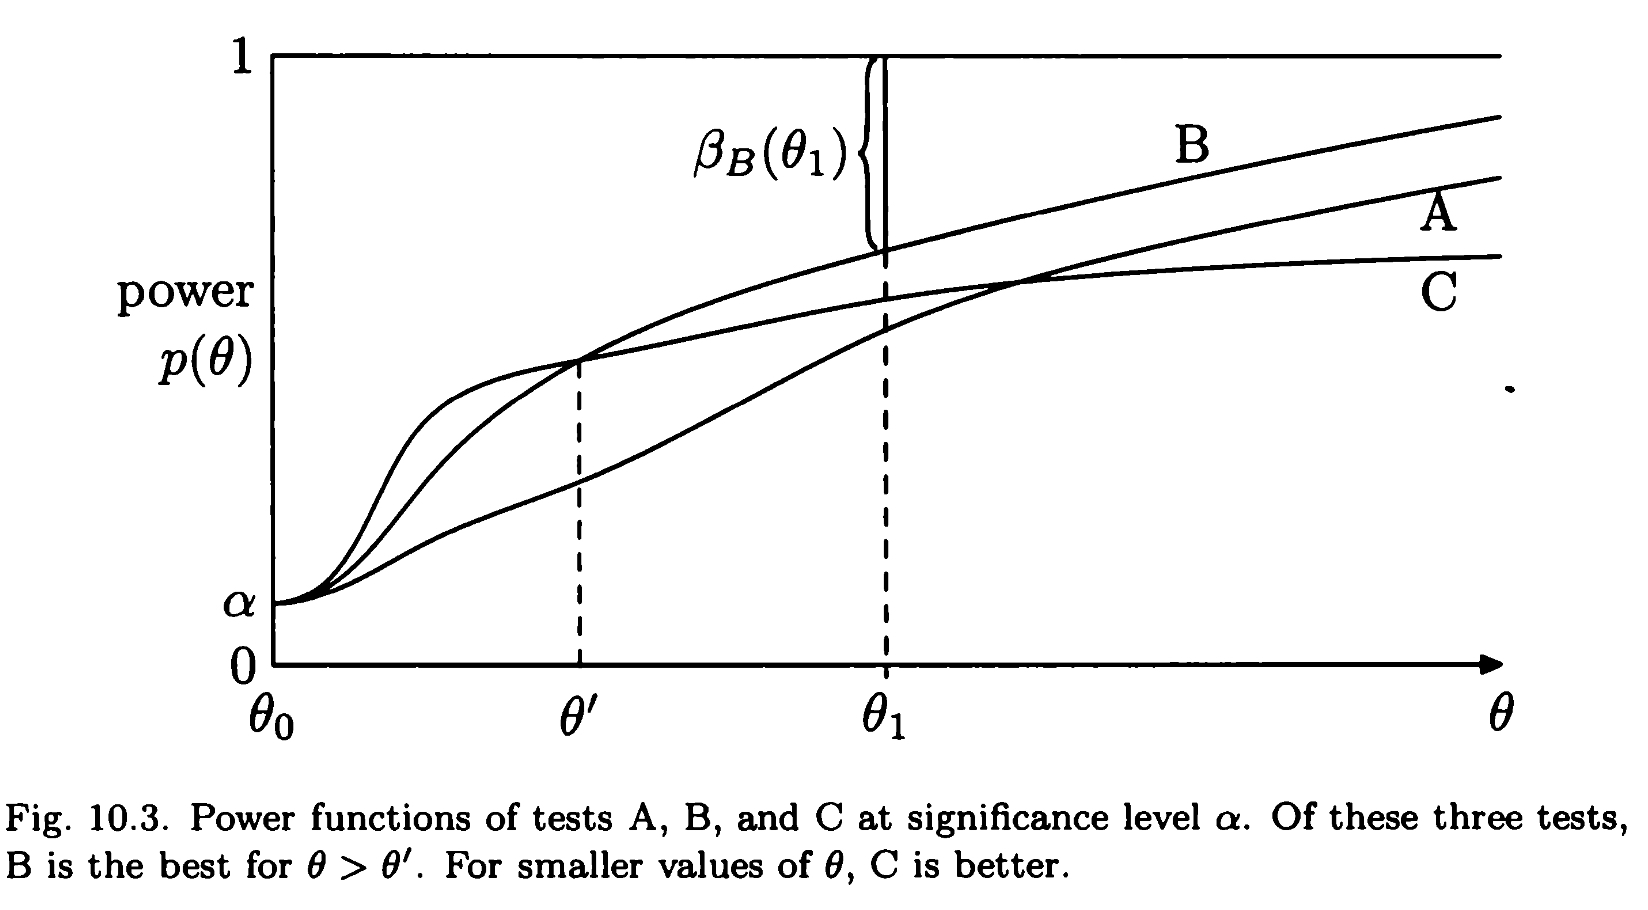
\includegraphics[trim={0cm 0cm 0 0},clip, keepaspectratio,width=0.85\textwidth]{mostpower}
	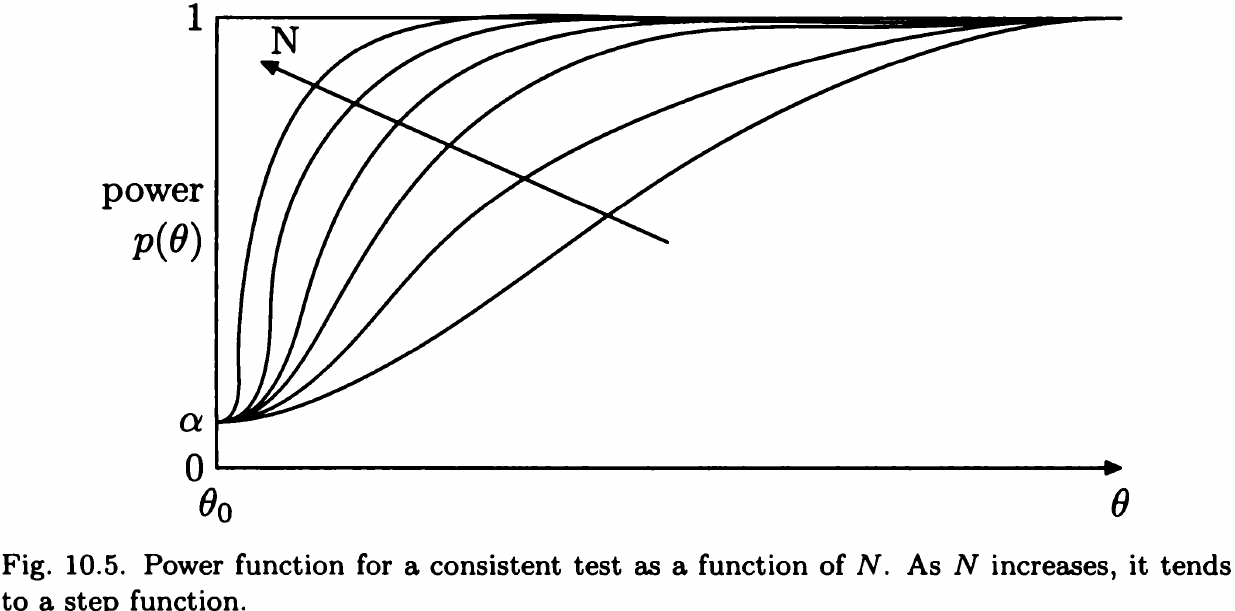
\includegraphics[trim={0cm 0 0 0},clip, width=0.85\textwidth]{powerconsistent}
	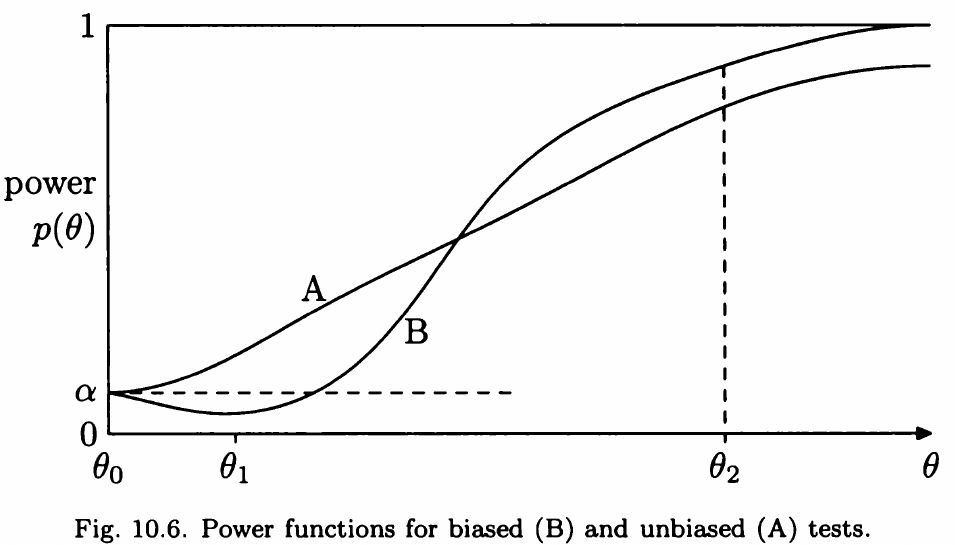
\includegraphics[trim={0cm 0 0 0},clip,width=0.8\textwidth]{biasedtest}
\end{figure} 
	Test B can't distinguish between $\theta_0$, $\theta_1$.
\end{column}
\end{columns}
\end{frame}

\begin{frame}{Ipotesi semplici: Lemma di Neyman-Pearson (Test di NP)}
Posso esprimere un test in funzione di una statistica: $T(\vec{x})=T(t(\vec{x}))$ (nel caso del lemma NP la statistica \'e il LR). 
Lo spazio dei parametri \'e $\theta_0,\theta_1$. Cerco la regione $w_{\alpha}$ regione critica che massimizza power $1-\beta$ (dato $\alpha$):
\begin{align*}
&\int_{w_{\alpha}}f_N(\vec{X}|\theta_0)\,dX=\alpha\\
&\int_{w_{\alpha}}f_N(\vec{X}|\theta_1)\,dX=1-\beta\\
&=\int_{w_{\alpha}}\frac{f_N(\vec{X}|\theta_1)}{f_N(\vec{X}|\theta_0)}f_N(\vec{X}|\theta_0)\,dX=\E_{w_{\alpha}}{[\frac{f_N(\vec{X}|\theta_1)}{f_N(\vec{X}|\theta_0)}|\theta_0]}\\
&\Rightarrow l_N(\vec{X},\theta_0,\theta_1)=\frac{f_N(\vec{X}|\theta_1)}{f_N(\vec{X}|\theta_0)}\geq c_{\alpha}: H_1\ (\leq c_{\alpha}: H_0)\\
&\int_{w_{\alpha}}=\{x:I_N>c_{\alpha}\}f(x,\theta_0)\,dx=\alpha
\end{align*}
\end{frame}

\begin{wordonframe}{Regione critica: NP, il verso della disuguaglianza e il quantile}
Voglio distinguere $H_0: G(\mu_0,\sigma)$ vs $H_1: G(\mu_1>\mu_0,\sigma)$ - Lemma NP:
\begin{align*}
&\frac{L(\mu_0)}{L(\mu_1)}=\exp{\frac{1}{2\sigma}[\sum_i(x_i-\mu_1)^2-\sum_i(x_i-\mu_0)^2]}\\
&C=\{(x_i):\exp{\frac{1}{2\sigma}[\sum_i(x_i-\mu_1)^2-\sum_i(x_i-\mu_0)^2]}\leq k\}\\
&C=\{(x_i):\exv{X}\geq k'=\mu_0+\lambda_{1-\alpha}\frac{\sigma}{\sqrt{N}}\}
\end{align*}
\end{wordonframe}

\begin{frame}{Ipotesi composte}
\begin{itemize}
\item Karlin-Rubin theorem: extension of NP lemma to composite H. Scalar measurement with pdf parametrized by scalar $\theta$, if $l(x)=\frac{f(x;\theta_1)}{f(x;\theta_0)}$ is monotone non-decreasing in $x$ for any pair $\theta_1\geq\theta_0$ then test for $H_0: \theta\leq\theta_0(\theta=\theta_0)$ vs $H_1: \theta>\theta_0$ defined by threshold test function $\phi(X)=\lbt{1\ x>x_0}{0\ x<x_0}$ con $\E_{\theta_0}{[\phi]}=\alpha$
\item For exponential family exists UMP one-sided ($H_0: \theta=\theta_0$, $H_1: \theta>\theta_0$)
\item Se non esiste UMP test e ho bisogno di massima sensibilit\'a in intorno di $\theta_0$: score \'e asintoticamente normale
\[\PDy{\theta}{\ln{L}}|_{\theta_0}\gtrless\lambda_{?1-\alpha}\sqrt{NI}\]
\end{itemize}
\end{frame}

\begin{frame}{LMP test}
Se ho bisogno di massima sensibilit\'a vicino alla soglia: $1-\beta$ grande nelle vicinanze di 0: $H_0$: $\theta=\theta_0$, $H_1$: $\theta=\theta_0+\Delta$, quindi $\ln{L(\vec{X},\theta_1)}\approx\ln{L(\vec{X},\theta_0)}+\Delta\PDy{\theta}{\ln{L}}|_{\theta_0}$.
Applico NP a $H_0$ vs $H_1$:
\begin{equation*}
\ln{L(\vec{X},\theta_1)}-\ln{L(\vec{X},\theta_0)}\gtrless c_{\alpha} \Rightarrow \PDy{\theta}{\ln{L}}\gtrless q_{\alpha}
\end{equation*}
\begin{columns}[T]
	\begin{column}{0.4\textwidth}
		\begin{align*}
		&H_0: \theta=\theta_0\\
		&H_1: \theta=\theta_0+\Delta
		\end{align*}
	\end{column}
	\begin{column}{0.6\textwidth}
		\begin{align*}
		&\PDy{\theta}{\log{L}}\gtrless k_{\alpha}\gtrless\lambda_{\alpha}\sqrt{NI}\\
		&\E{[\PDy{\theta}{\log{L}}|_{\theta_0}]}=0,\ \E{[(\PDy{\theta}{\log{L}}|_{\theta_0})^2]}=NI
		\end{align*}
	\end{column}
\end{columns}
\end{frame}

\begin{frame}{LR test}
James pg 287
\end{frame}

\section{GOF}

\subsection{Binned GOF}

\begin{frame}{Pearson $\chi^2$ test for multinomial null hypothesis (histograms with k bins)}
Asymptotic normality of multinomial to find asymptotic pdf of
\[(\vec{n}-N\vec{p})^T\invers{V}(\vec{n}-N\vec{p})\]
$V$ matrice covarianza osservazioni $\vec{n}$ di rango $k-1$ visto $\sum_i^kn_i=N$. Treating all bins simmetrically we find
\[T=\frac{1}{N}\sum_i^k\frac{(n_i-Np_i)^2}{p_i}\]
distribution of T close enough to $\chi^2(k-1)$ when all expected events per bin $Np_i>5$
\end{frame}

\begin{wordonframe}{Dettagli su $\chi^2$ di pearson}
$k+1$ outcomes, n trials, $\sum_jp_j=1$, $\sum_in_i=N$: $\prob{(Y_1=y_1,\ldots,Y_{k+1}=y_{k+1})}=\frac{n!}{y_1!*\ldots*y_{k+1}!}p_1^{y_1}\ldots p_{k+1}^{y_{k+1}}$. Parameter space $\Omega=\{(p_1,\ldots,p_k\})\in \real{k}: p_i\geq0,\sum_{j=1}^kp_j\leq1$.
$H_0: p_i=\pi_i$ vs $K: p_i\neq\pi_i$:
statistica $Q_n=\sum_j^{k+1}\frac{(Y_j-n\pi_j)^2}{n\pi_j}\to\frac{1}{N}\sum^{k+1}\frac{n_i^2}{p_i}-N$ ha asintotic. pdf $\chi^2(k)$, quindi se $c_{k,1-\alpha}$ $1-\alpha$-quantile di $\chi^2(k)$ il test che rifiuta H quando $Q_n>c_{k,1-\alpha}$ ha asintoticamente valore critico $\alpha$.
\begin{block}{Power against local alternatives}
	\begin{itemize}
		\item $H: p_j=\pi_j$, $j=1,\ldots,k+1$: $Q_n\xrightarrow{d}\chi^2(k)$
		\item Under alternative hypothesis $K: p_j^{(n)}=\pi_j+n\expy{-1/2}h_j$, $\sum_jh_j=0$: $Q_n\xrightarrow{d}\chi^{2,\lambda}(k)$ and NC parameter $\lambda=\sum_j^{k+1}\frac{h_j^2}{\pi_j}$
		\item Power of $\chi^2$ test based on $Q_n$ tends to a limit greater than critical value $\alpha$
	\end{itemize}
\end{block}
\end{wordonframe}

\begin{frame}{$\chi^2$ Test of uniformity}
$X_1,\ldots,X_n$ iid RV con pdf $F$; $H: F=F_0(t)=t$ uniform cdf in $(0,1)$. Divido l'intervallo $(0,1)$ in $k+1$ sotto-intervalli di lunghezza $\frac{1}{k+1}$: pdf di $(Y_1,\ldots,Y_{k+1})$ \'e multinomiale e il test che rifiuta H per grandi $\sum_j^{k+1}\frac{(Y_j-\frac{n}{k+1})}{\frac{n}{k+1}}$.
\end{frame}

\subsection{Unbinned GOF}

\begin{frame}{Kolmogorov-Smirnov and Cramer-von Mises tests}
\begin{block}{Classes of EDF statistics}
	Empirical distribution function (EDF): N iid RV: $F_n(X)=\frac{1}{N}\sum_i^NI_{[-\infty,x](X_i)}$ $\hat{F}_n(t)=\frac{\#\text{ elementi nel campione }\leq t}{n}$.
 Ordering statistics, $X_{(1)}, X_{(2)}, \ldots X_{(N)}$, $S_N=\left\{\begin{array}{c}0\ X<X_{(1)}\\i/N\ X_{(i)}<X<X_{(i+1)}\\1\ X>X_{(N)}\end{array}\right\}$
\end{block}
%Smirnov-Cramer-von Mises test for unbinned data

\begin{block}{Test di Kolmogorov-Smirnov }
La statistica \'e massima deviazione di $S_N$ osservato da distribuzione $F(X)$ sotto $H_0$:
\begin{align*}
&D_N=\max|S_N(X)-F(X)|:\ \lim_{N\to\infty}\prob{[\sqrt{N}D_N>z]}=2\sum_{r=1}^{\infty}(-1)\expy{r-1}\exp{-2r^2z^2}\\
&D_N^{\pm}=\max\pm(S_N(X)-F(X)):\ \lim_{N\to\infty}\prob{[\sqrt{N}D_N^{\pm}>z]}=\exp{-2z^2}
\end{align*}
%$T_n=\sup_{t\in\real}{|\hat{F}_n(t)-F(t)|}$: largest of $|F_n(y_k)-F_0(y_k)|$, $|F_n(y_{k-1})-F_0(y_k)|$. Sia $s_{n,1-\alpha}$ il $1-\alpha$-quantile di $T_n$ per ogni $F$ continua: KS-test rejects H if $T_n>s_{n,1-\alpha}$.
Rejects null hypothesis at level $\alpha$ if $\sqrt{N}D_N>K_{\alpha}$ dove $K_{\alpha}$ \'e determinato tramite $\prob{[\sqrt{N}D_N<K_{\alpha}]}=1-\alpha$ (asintoticamente)
\end{block}
\end{frame}


\section{Compiti}\linkdest{compiti}

\begin{frame}[allowframebreaks]{Section TOC}
%currentsection,hideallsubsections,subsubsectionstyle=hide
\tableofcontents[currentsection,sectionstyle=show/hide,subsectionstyle=show/show/hide]
\end{frame}

\subsection{{Combinazione p-value per 10 osservabili indipendenti (16/07/18)}}
\begin{frame}{Valori $\chi^2$ per 10 osservabili binned}
	Fit di massima likelihood per le 10 osservabili (binned) basandosi su teoria: istogrammi suff. popolati per GOF test di Pearson con 30 dof (31 bins?)
	\begin{table}[h!]
		\centering
		\begin{tabular}{||cccccc||} 
			$\chi^2(/30?)$&38.33&40.87&30.70&36.91&39.97\\
			&36.97&20.48&32.34&41.32&41.41\\
			$P(\chi^2_{30}<x)$&0.859&0.911&0.570&0.820&0.894\\
			&0.822&0.096&0.648&0.918&0.920\\
		\end{tabular}
	\end{table}
	Impressione che ci siano troppi valori alti del $\chi^2$: come risolvere il dubbio in maniera rigorosa?
\end{frame}
\begin{frame}{Additivit\'a $\chi^2$ e GOF test}
	\begin{itemize}
	\item \keyword{additivit\'a del $\chi^2$}: somma quadrati di RV normali standard.
			Sommando $\chi^2$ in tab si ottiene RV con pdf $\chi^2_{300}$ approssimabile con gaussiana con $\sigma=\sqrt{2N}\approx24.5$.
			$\sum_i\chi^2_i=359.3$, siamo a $1.21\sigma$
	\item KS test: campione di 10 valori in accordo con pdf $\chi^2_{30}$ (cumulante $\prob{(\chi^2_{30}<x)}$ in tabella). Calcolo $F_n(x_{k-1})-F_n(x_k)$ e $F_n(x_k)-F_n(x_k)$:  $|0-0.096|$, $|0.1-0.57|$, $|0.2-0.648|$, $|0.3-0.82|$, $|0.4-0.822|$, $|0.5-0.859|$, $|0.6-0.894|$, $|0.7-0.914|$, $|0.8-0.918|$, $|0.9-0.926|$; $\Delta=0.52$??
	\item Combinazione diretta p-values: $p_i=1-\prob{(\chi^2_{30}<x)}$, pdf somma log p-values $-2\log{(\prod^Np_i)}$ ha pdf $\chi^2_{2N}$
	\item Test binned: hist of p-values (3-4) e considero LR con pdf uniforme (pdf p-value) e quindi usarlo per test basato su pdf asintotica (esatta, calcolandola)
	\item Considerare max(min) dei p-values e usare pdf $x_M$ per test
	\item Test della mediana
	\item Test basato su propriet\'a pdf $\chi^2_{30}$: test varianza $2N$; test secondo momento attorno a media nominale 30.
\end{itemize}
\end{frame}

\begin{frame}{Stimatori, confidence/credible interval per parametro m di pdf uniforme da misura della mediana(16/07/18)}
\begin{columns}[T]\begin{column}{0.5\textwidth}
x RV $U(0,m)$; $2k+1=3$ misura la mediana $x_2=3.4$
\begin{block}{MLE estimator, bias, incertezza statistica}
\begin{align*}
&\prob{(\mu=x_2)}=6\frac{\mu}{m^2}(1-\frac{\mu}{m})\\
&\hat{\mu}_{MLE}=3/2\mu\\
&\E{[\hat{m}]}=\frac{3}{2}\E{[\mu]}\frac{3}{2}\int_0^{m}\mu\prob{(\mu)}\,d\mu\\
&=\frac{3}{4}m\\
&\hat{m}'=\frac{4}{3}\hat{m}=2\mu\\
&\var{[\hat{m}]}=\sigma^2_{\hat{m}}=\frac{9}{4}\var{\mu}=\frac{9}{4}\sigma_{\mu}^2\\
&\var{[\hat{m}']}=\sigma^2_{\hat{m}'}=4\var{\mu}=4\sigma_{\mu}^2\\
&\sigma^2_{\mu}=\exv{\mu^2}-\exv{\mu}^2=\frac{m^2}{20}
\end{align*}
Le varianze sono funzione del valore di m: le stimo usando $\hat{m}$
\end{block}
\end{column}\begin{column}{0.5\textwidth}
Likelihood pdf uniforme: \begin{equation*}L_x(m)=\left\{\begin{array}{c}
0\ m<x\\
1/m\ m\geq x\\
\end{array}\right.
\end{equation*}
Determinazione $p(\mu=x_2)$ dove $\mu$ pu\'o essere vista come seconda misura pi\'u grande o mediana; per $2k+1$ misure
\begin{align*}
&\prob{(\mu;m)}=\prob{(\mu)}F(\mu)^k[1-F(\mu)]^k\\
&(2k+1)\binom{2k}{k}\\
&\prob{(\mu;m)}=\frac{1}{m}(\frac{\mu}{m})^k(1-\frac{\mu}{m})^k\frac{(2k+1)!}{k!k!1!}
\end{align*}
\vspace{5cm}
\begin{block}{Stima bayesiana di m}
Assumo prior uniforme in $\log{m}$: $\prob{(m)}\propto\frac{1}{m}$, posterior $\pi(m)\propto L(\mu|m)\prob{(m)}=\frac{6\mu}{m^3}-\frac{6\mu^2}{m^4}$ ($\prob{(H)}=\frac{\prob{(E|H)\prob{(H)}}}{\prob{(E)}}$): la posterior va normalizzata tra $[\mu,+\infty]$ (likelihood nulla  in $[0,\mu]$), $\pi(m)=\frac{3\mu^2}{m^3}-\frac{3\mu^3}{m^4}$, il massimo fornisci una stima bayesiana di m: $\hat{m}=\frac{4}{3}\mu$.
\end{block}
\end{column}\end{columns}
\end{frame}

\begin{frame}{Stimatori, confidence/credible interval per parametro m di pdf uniforme da misura della mediana(16/07/18)}
\begin{columns}[T]\begin{column}{0.5\textwidth}
\begin{block}{MLE estimator, bias, incertezza statistica}
\begin{align*}
&\var{[\hat{m}']}=\sigma^2_{\hat{m}'}=4\var{\mu}=4\sigma_{\mu}^2\\
&\sigma^2_{\mu}=\exv{\mu^2}-\exv{\mu}^2=\frac{m^2}{20}
\end{align*}
Le varianze sono funzione del valore di m: le stimo usando $\hat{m}$
\end{block}
\end{column}\begin{column}{0.5\textwidth}
\begin{block}{Stima bayesiana di m}
Assumo prior uniforme in $\log{m}$: $\prob{(m)}\propto\frac{1}{m}$, posterior $\pi(m)\propto L(\mu|m)\prob{(m)}=\frac{6\mu}{m^3}-\frac{6\mu^2}{m^4}$ ($\prob{(H)}=\frac{\prob{(E|H)\prob{(H)}}}{\prob{(E)}}$): la posterior va normalizzata tra $[\mu,+\infty]$ (likelihood nulla  in $[0,\mu]$), $\pi(m)=\frac{3\mu^2}{m^3}-\frac{3\mu^3}{m^4}$, il massimo fornisci una stima bayesiana di m: $\hat{m}=\frac{4}{3}\mu$.
\end{block}
\end{column}\end{columns}
\end{frame}

\begin{frame}{Limite di confidenza superiore/bilaterale}
Limite superiore per m di $U(0,m)$ da mediana campionaria: $\int_{\mu}^m6\frac{\tilde{\mu}}{m^2}(1-\frac{\tilde{\mu}}{m})\,d\tilde{\mu}=\cl=0.9$, con $y=\frac{\mu}{m}$ si risolve $F(\mu)=y^2(3-2y)=1-\cl$ ha soluzione $y=0.1958$ quindi $m<\frac{\mu}{0.1958}$.
Limite bilaterali simmetrici per m da mediana campionaria: $F(\mu)=y^2(3-2y)=(1-\cl)/2$ $y_+=0.13535$, $\int_{\mu}^m6\frac{\tilde{\mu}}{m^2}(1-\frac{\tilde{\mu}}{m})\,d\tilde{\mu}=(1-\cl)/2$ quindi $F(\mu)=y^2(3-2y)=(1+\cl)/2$ e $y_-=0.8647$: Limiti bilaterali con $\cl=0.9$ sono $\frac{\mu}{0.8647}<m<\frac{\mu}{0.13535}$
\end{frame}

\begin{frame}{Limiti credibilit\'a Bayesiana}
prior uniform, $\cred=90\%$. La posterior \'e $\pi(m)=\frac{2\mu}{m^2}-\frac{2\mu^2}{m^3}$ diversa da zero in $[\mu,+\infty]$ e la cumulante $F(m)=\int_{\mu}^m\pi(\tilde{m})\,d\tilde{m}=1+\mu(\frac{\mu}{m^2}-\frac{2}{m})$:
\begin{align*}
&F(m_{min})=\frac{1-\cl}{2}\\
&F(m_{max})=\frac{1+\cl}{2}\\
&\frac{\mu}{1-\sqrt{(1-\cl)/2}}<m<\frac{\mu}{1-\sqrt{(1+\cl)/2}}
\end{align*}
dove ho scelto le soluzioni maggiori di $\mu$, per il limite superiore si ha $m<66.26$.
\end{frame}

\begin{frame}{Limiti confidenza al $90\%\cl$ \'a l\'a FC}
Imponiamo il LR-ordering e coverage $90\%$
\begin{equation*}
\lambda\propto\mu\prob{(\mu;m)}=6\frac{\mu^2}{m^2}(1-\frac{\mu}{m})
\end{equation*}
LR \'e unimodale: un intervallo con $\lambda(m_1)=\lambda(m_2)$, mentre il coverage richiede $\int_{m_1}^{m_2}\prob{(\mu;m)}\,d\mu=\cl$ da cui si ottiene il sistema di equazioni
\begin{align*}
&y_2^3-y_1^3=\cl\\
&y_2^2-y_1^2=\cl\\
&y_1=\frac{m_1}{m},\ y_1=\frac{m_1}{m}\\
&\frac{\mu}{0.96804}<m<\frac{\mu}{0.192606}
\end{align*}
\end{frame}

\begin{frame}{$2k+1$ misure: propriet\'a statistica mediana per costruzione estimatori}
pdf per mediana campionaria
\begin{equation*}	\prob{(\mu;m)}=\frac{1}{m}(\frac{\mu}{m})^k(1-\frac{\mu}{m})^k\frac{(2k+1)!}{k!k!1!}
\end{equation*}
stimatore massima likelihood:
\begin{align*}
&\log{L(m)}=\log{\frac{1}{m}}+k\log{\frac{\tilde{m}}{m}}+k\log{(1-\frac{\tilde{m}}{m})}+\const{}\\
&\TDy{m}{\log{L}}=0 \Rightarrow \hat{m}=\frac{2k+1}{k+1}\tilde{m}
\end{align*}
Bias estimatore:
\begin{align*}
&\E{[\hat{m}]}=\frac{2k+1}{k+1}\E{[\tilde{m}]}\\
&\E{[\tilde{m}]}=\int_0^m\tilde{m}\prob{(\tilde{m};m)}\,d\tilde{m}\\
&=\frac{(2k+1)!}{k!k!1!}m\int_0^1x^{k+1}(1-x)^k\,dx\ (x=\frac{\tilde{m}}{m})\\
&\E{[\tilde{m}]}=\frac{(2k+1)!}{k!k!1!}m\frac{\Gamma(k+1)\Gamma(k+2)}{\Gamma(2k+3)}=\frac{m}{2}\ (\Gamma(k+1)=k!)\\
&\E{[\hat{m}]}=\frac{2k+1}{2(k+1)}m\\
&b=m-\frac{2k+1}{2(k+1)}=\frac{1}{2(k+1)}m\to0
\end{align*}
Varianza
\begin{align*}
&\E{[\tilde{m}^2]}=\frac{(2k+1)!}{k!k!1!}m^2\int_0^1x^{k+2}(1-x)^k\,dx\\
&=\frac{(2k+1)!}{k!k!1!}m^2\frac{\Gamma(k+1)\Gamma(k+3)}{\Gamma(2k+4)}\\
&=\frac{(k+1)(k+1)}{(2k+3)(2k+2)}m^2\\
&\var{[\tilde{m}]}=\E{[\tilde{m}^2]}-\E{[\tilde{m}]}^2=m^2\frac{1}{4(2k+3)}\\
&\var{[\hat{m}]}=(\frac{2k+1}{k+1})^2\var{[\tilde{m}]}\to0
\end{align*}
Efficienza estimatore mediana campionaria per pdf uniforme: non si pu\'o usare MVB come riferimento assoluto dato che per pdf uniforme $I_F$ non \'e proporzionale al numero di misure; efficienza relativa rispetto a stimatore ricavato da statistica suff. $x_M$ $\var{[x_M]}=frac{m^2}{k^2}$: il MLE ricavato da mediana \'e meno efficiente ed efficienza relativa va a 0.
\end{frame}

\subsection{Stime limite superiore dati da pdf uniforme (Problema 1 - Compito $09/11/18$)}

\begin{frame}{Pdf secondo valore pi\'u grande $x_2$}
pdf di $X_{(2)}$ per N estrazioni da pdf uniforme:
\begin{align*}
&\prob{(X_{(k)}<x)}=\sum_{i=k}^nc(n,i)F(x)^i[1-F(x)]^{n-i}\\
&\PDof{p}\sum_{i=k}^nc(n,i)p^{i}[1-p]^{n-i}=nC(n-1,k-1)p\expy{k-1}(1-p)\expy{k-1}\\
&\prob{(X_{(k)})}=nC(n-1,k-1)f(x)F(x)\expy{k-1}(1-F(x))\expy{k-1}\\
&\prob{(x_2;m)}=N(N-1)\frac{1}{m^N}x_2\expy{N-2}(m-x_2)
\end{align*}
\end{frame}

\begin{frame}{Confronto efficienza stimatore da $x_2$ vs $x_M$}
\begin{columns}[T]
\begin{column}{0.5\textwidth}
Efficienza stimatore di m da statistica $x_2$:\\
Massimizzando $L(m)$ per m si ha $\hat{m}=\frac{N}{N-1}x_2$\\
bias $\E{[\hat{m}]}-m=-\frac{1}{N+1}m$:\\ $\hat{m}'=\frac{N+1}{N}\hat{m}=\frac{N+1}{N-1}x_2$\\
varianza $\var{[\hat{m}']}=\E{[\hat{m}'^2]}-\E{[\hat{m}']}^2$
\begin{align*}
&\E{[\hat{m}'^2]}=\frac{(N+1)^2}{(N-1)^2}\E{[x_2^2]}\\
&=\frac{2}{(N-1)(N+2)}m^2
\end{align*}
\end{column}
\begin{column}{0.5\textwidth}
Efficienza $x_M$:\\
$\hat{m}_{MLE}=x_M$, stimatore unbiased $\hat{m}'=\frac{N+1}{N}\hat{m}$:
\begin{align*}
&\prob{(x_M)}=\frac{N}{m}(\frac{x_M}{m})^{N-1}\\
&L_{x_M}(m)=I_{x>M}\frac{1}{m}
\end{align*}
varianza di $\hat{m}'$:
\begin{align*}
&\E{[\hat{m}'^2]}-\E{[\hat{m'}]}^2=\frac{(N+1)^2}{N^2}\frac{N}{N+2}m^2-m^2\\
&=\frac{1}{N(N+2)}m^2
\end{align*}
efficienza relativa
\begin{equation*}
\epsilon_r=\frac{\var{[\hat{m'}_{M}]}}{\var{[\hat{m'}_{x_2}]}}
\end{equation*}
\end{column}
\end{columns}
\end{frame}

\begin{frame}{Ripetizione misure $x_2$}
Combinazione likelihood 2 misure di $x_2$: MLE massimizzando likelihood combinata
\begin{align*}
&L(m_1,m_2;x_2'x_2'')=N^2(N-1)^2\frac{1}{m^{2N}}{x_2'}^{N-1}{x_2''}^{N-2}(m-x_2')(m-x_2'')\\
&2(N-1)m^2+(x_2'+x_2'')(2N-1)m-2N(x_2'x_2'')=0\\
&\hat{m}_{\pm}=\frac{(x_2'+x_2'')(2N-1)\pm\sqrt{(x_2'+x_2'')^2(2N-1)^2-16N(N-1)x_2'x_2''}}{4(N-1)}
\end{align*}
Asintoticamente $\hat{m}=\max{(x_2',x_2'')}$ (Assumo $x_2''>x_2'$)
\end{frame}

\begin{frame}{Monotone LR}
Test bilaterale di ipotesi composte: dati da pdf uniforme con $m_1\neq m_2$? \\
Likelihood ratio test:
\begin{equation*}
\lambda(x_1',x_2'')=-2\log{\frac{\sup_m{p(x_2',x_2'';m)}}{\sup_{m_1,m_2}{p(x_2',x_2'';m_1,m_2)}}}
\end{equation*}

\begin{align*}
&\hat{m}=f(N)x_2\Rightarrow p(x_2',\hat{m})=G(N)/x_2',\ p(x_2'',\hat{m})=G(N)/x_2''\\
&\sup_{m_1,m_2}{p(x_2',x_2'';m_1,m_2)}\propto\frac{1}{x_2'x_2''},\ p(x_2',x_2'';m)\propto(m-x_2')(m-x_2'')(x_2'x_2'')^{N-2}\\
&??\sup_{m}p(x_2',x_2'';m)\propto x_2''(x_2''-x_2')(x_2'x_2'')^{N-2}
\end{align*}
Likelihood ratio monotona (asintoticamente): statistica $t(x_2',x_2'')=x_2''/x_2'$: il test LR \'e della forma $x_2''/x_2'>q_{\alpha}$
Monotone LR in statistic $T(x)$ and Karlin-Rubin theorem
\end{frame}

\subsection{Stima di tempo medio tra eventi di onde gravitazionali - problema 2 Compito $09/11/18$}

\begin{frame}{Pdf tempo tra eventi Poissoniani: MLE per eventi che generano onde gravitazionali - propriet\'a dello stimatore per numero eventi annuali}

Conteggi generati da eventi casuali statisticamente indipendenti: distribuzione del tempo tra due eventi (Poissoniana con $n\approx1$) esponenziale $\prob{(t;\tau)}=\frac{1}{\tau}\exp{-\frac{t}{\tau}}$. Il massimo della likelihood ci fornisce stimatore $\hat{t}=t_m=\SI{39}{\day}$ quindi ha la stessa distribuzione esponenziale dei tempi t: $\E{[\hat{\tau}]}=\tau$, $\var{[\tau]}=\tau^2$ quindi $\hat{\tau}=\SI{0.107+-107}{\year}$.
Il MLE trasforma in modo banale sotto cambio di variabile: $\hat{\lambda}=\hat{\frac{1}{\tau}}=\SI{9.3}{\counts\per\year}$; usando formula per propagazione errori si ha
\begin{equation*}
\sigma(\lambda)=\sqrt{\var{[\hat{\lambda}]}}\approx\frac{1}{\tau^2}\sqrt{\var{[\tau]}}
\end{equation*}
Tuttavia l'approssimazione quasi lineare del cambio di variabile \'e una pessima approssimazione sull'ampio intervallo di incertezze della variabile originale.
La distribuzione di $\hat{\lambda}=\frac{1}{\hat{\tau}}$ \'e:
\begin{equation*}
\prob{(\hat{\lambda},\lambda)}=\prob{(\hat{\tau}(\hat{\lambda});\lambda=\frac{1}{\tau})}|\TDy{\hat{\lambda}}{\hat{\tau}(=\frac{1}{\hat{\lambda}})}|
\end{equation*}
Momenti di ordine $>0$ non esistono: $\var{[\lambda]}=\infty$.
\end{frame}

\begin{frame}{Limiti di confidenza su numero eventi annuali: p-ordering, limite inferiore, LR-ratio di $\lambda$}

Stima intervallare di $\lambda=\frac{1}{\tau}$ e $\prob{(t;\lambda)}=\lambda\exp{-\lambda t}$: pdf \'e monotona decrescente in t quindi p-ordering equivale a $o(t)=-t$, $t\leq t_{max}(\lambda)$
\begin{align*}
&\int_0^{t_{max}}\lambda\exp{-\lambda t}\,dt=\cl{}:\ t_{max}(\lambda)=-\frac{\log{(1-\cl{})}}{\lambda}
\end{align*}
$t_{max}(\lambda)$ decrescente in $\lambda$, da $t<t_{max}(\lambda)$ si vede che la banda di confidenza \'e della forma $t<t_{max}(\lambda)$ porta a limite $\lambda\leq\lambda_{max}$ (limite superiore); l'inversione porta a $\lambda_{max}=-\frac{\log{(1-\cl{})}}{t_m}$.
Ma limite inferiore a un fenomeno nuovo! $o(t)=t$:
\begin{equation*}
\int_{t_{min}}^{\infty}\lambda\exp{-\lambda t}\,dt=\cl{}\Rightarrow t_{min}(\lambda)=-\frac{\log{(\cl{})}}{\lambda}
\end{equation*}
banda della forma $t\geq t_{min}(\lambda)$ porta, essendo $t_{min}(\lambda)$ decrescente il $\lambda$, a limite inferiore $\lambda\geq\lambda_{min}=-\frac{\log{(\cl{})}}{t_m}$. 

LR-ordering:
\begin{equation*}
\lr{}=\frac{\prob{(t;\lambda)}}{\sup_{\lambda}\prob{(t;\lambda)}}=\lambda t\exp{-\lambda t}
\end{equation*}
fissato $\lambda$ ha singolo massimo in t e monotona da ambo i lati: usando $o(t)=\lr{(t)}$ ottengo intervallo $[t_{min},t_{max}]$.
\end{frame}

\begin{frame}{Limiti di credibilit\'a (Bayesiani)}
Prior impropria: in mancanza di una scala definita utilizzo prior uniforme in $[0,\infty]$ (non normalizabile). Devo normalizare la posterior:
\begin{align*}
&\pi(\lambda|t_m)\propto \lambda\exp{-t_m\lambda}=L_{t_m}(\lambda)\\
&\pi(\lambda|t_m)=t_m^2\lambda\exp{-t_m\lambda}
\end{align*}
\begin{columns}[T]
	\begin{column}{0.5\textwidth}
Limite bayesiano inferiore
\begin{equation*}
\int_{\lambda_{min}}^{\infty}t_m^2\lambda\exp{-t_m\lambda}\,d\lambda=\cl{}
\end{equation*}
	\end{column}
	\begin{column}{0.5\textwidth}
Limite bayesiano bilaterale simmetrico:
\begin{align*}
&\int_0^{\lambda_{min}}t_m^2\lambda\exp{-t_m\lambda}\,d\lambda=\frac{1-\cl}{2}\\
&\int_{\lambda_{max}}^{\infty}t_m^2\lambda\exp{-t_m\lambda}\,d\lambda=\frac{1-\cl}{2}
\end{align*}
\end{column}
\end{columns}
Limite bayesiano utilizzando posterior ordering:
\begin{align*}
&\exp{-t_m\lambda_{min}}(t_m\lambda_{min}+1)-\exp{-t_m\lambda_{max}}(t_m\lambda_{max}+1)=\cl\\
&\lambda_{min}\exp{-t_m\lambda_{min}}-\lambda_{max}\exp{-t_m\lambda_{max}}=0
\end{align*}
\end{frame}

\subsection{Modello goal fatti durante partita come realizzazione poissoniana - Compito del $10/09/18$}

\begin{frame}{Modello di partita di calcio - approccio Bayesiano per determinare probabilit\'a della forzo di una squadra e del risultato successivo}
Probabilit\'a che squadra A faccia gol in un minuto \'e $q_A$: la probabilit\'a che un'incontro A-B finisca $g_A-g_B$ \'e
\[P(g_ag_B=\exp{-\mu_A-\mu_B})\frac{\mu_A\expy{g_A}\mu_B\expy{g_B}}{g_A!g_B!}\] con $\mu_i=90*q_i$.
Sia un risultato $(0,1)$: utilizzo approccio bayesiano per determinare la probabilit\'a della ''forza'' della squadra
\[\pi(g_A,g_B)=L_{0-1}(g_A,g_B)p(g_A)p(g_B)\propto\mu_2\exp{-(\mu_1+\mu_2)}\]
La probabilit\'a $P(q_A>q_B)$ integro la posterior su $dq_Adq_B$ sopra la retta $q_A=q_B$. Per determinare la probabilit\'a che in successivo incontro si abbia uno $0-0$ o $1-0$ uso la posterior calcolata in seguito allo $0-1$ che pesa le poissoniane integrati sui valori dei parametri:
\[P(g_A,g_B)=\int P(g_A,g_B;\mu_1,\mu_2)\pi(\mu_1,\mu_2)\,d\mu_1\,d\mu_2\]
\end{frame}

\begin{frame}{Test verifica modello con LRT e $\chi^2$-Pearson}
La verifica del modello tramite il confronto con risultati di 3 partite per squadra con 8 squadre: quindi confronto l'ipotesi che i gol fatti nelle tre partite da una squadra appartengano a singola Poissoniana con un modello in cui ogni risultato viene da Poisson diversa:
\[\lambda=-2\log{LR}=2\sum g_{ij}\log{\frac{g_{ij}}{\exv{g_i}}}\]
$\prob{(\lambda)}\to\chi^2_{16}$ (24-8=8*(3-1)); usando il test di Pearson $\chi^2=\sum_{ij}\frac{g_{ij}-\exv{g_i}}{\exv{g_i}}$
\end{frame}

\subsection{Contaminazione radioattiva - Compito del $10/09/18$}

\begin{frame}{Determino livello contaminazione $\alpha$ da conteggi nel tempo}
$^{32}P$, $t_{1/2}^{32}=\SI{14.263}{\day}$ di cui voglio misurare livello contaminazione $\alpha$ con isotopo raro $^{33}P$, $t_{1/2}^{33}=\SI{25.25}{\day}$. Misuro conteggi particelle beta con rivelatore a stessa ora del giorno per 5 giorni $\{n_1,\ldots,n_5\}$.\\
Ignorando fattori dipendenti solo dai dati
\begin{align*}
&\log{L(N_0,\alpha)}=\sum_{i=1}^5(n_i\log{\mu_i(N_0,\alpha)}-\mu_i(N_0,\alpha))\\
&\mu_i(N_0,\alpha)=N_0[(1-\alpha)\lambda\exp{-\lambda t_i}+\alpha\lambda'\exp{-\lambda't_i}]
\end{align*}
\end{frame}

\begin{frame}{Likelihood equation e stima con 2 conteggi}
Le likelihood equations per determinare stimatore $\hat{\alpha}$:
\begin{align*}
&\PDy{N_0}{\log{L(N_0,\alpha)}}=\sum_{i=1}^5(\PDy{N_0}{\mu_i}[\frac{n_i-\mu_i}{\mu_i}])=0\\
&\PDy{\alpha}{\log{L(N_o,\alpha)}}=\sum_{i=1}^5(\PDy{N_0}{\mu_i}[\frac{n_i-\mu_i}{\mu_i}])=0
\end{align*}
i conteggi hanno pdf Poisson centrata attorno al valore atteso determinato da numero atomi radioattivi al momento della misure, il rate di decadimento, la durata della misura e l'efficienza del rivelatore; $N_0$ \'e un nuissance parameter.
\end{frame}

\begin{frame}{Stmatori usando momenti da sequenza temporale discreta}
Risolvere seconda equazione equivale a risolvere quinto grado che \'e fattibile in generale con metodi numerici; dato che ho da determinare 2 parametri considero solo 2 misure - prima e l'ultima - quindi si ha il sistema $n_1=\mu_1$ e $n_5=\mu_5$ per la varianza considero la propagazione della varianza (su $n_1$, $n_5$).
Adesso considero la distribuzione delle misure come sequenza temporale discreta e applico il metodo dei momenti per estrarre stima contaminazione ($t_i=i-1=0,\ldots,4$):
\[P(t_i;\alpha)\propto[(1-\alpha)\lambda\exp{-\lambda t_i}+\alpha\lambda'\exp{-\lambda't_i}]\]
Q normalizzazione, i momenti di ordine zero e uno:
\begin{align*}
&\mu_0(\alpha))=Q\sum_i^5[(1-\alpha)\lambda\exp{-\lambda t_i}+\alpha\lambda'\exp{-\lambda't_i}]\\
&\mu_1(\alpha))=Q\sum_i^5[(1-\alpha)t_i\lambda\exp{-\lambda t_i}+\alpha t_i\lambda'\exp{-\lambda't_i}]
\end{align*}
si ricavano i 2 parametri uguagliando i valori attesi e osservati:
\begin{align*}
&\E{[\mu_0]}=\sum_i^5n_i\\
&\E{[\mu_1]}=\sum_i^5(i-1)n_i
\end{align*}
\end{frame}

\section{Math tools}

\begin{frame}{algebra basic}

\begin{align*}
&4a(ax^2+bx+c)=0\\
&4a^2x^2+4abx+4ac+b^2-b^2=0\\
&(2ax+b)^2=b^2-4ac
\end{align*}
%McLAurin expansion
%
\end{frame}

\begin{wordonframe}{Espansioni di Taylor}
	\begin{align*}
	&\phi(t)=1+it\mu-\frac{\sigma^2t^2}{2}+o(t^2)\\
	&\log{(1+x)}\approx x-\frac{x^2}{2}+o(x^2)
	\end{align*}
\end{wordonframe}

\begin{frame}{Integrals}
\begin{columns}[T]\begin{column}{0.5\textwidth}

\end{column}\begin{column}{0.5\textwidth}
\end{column}\end{columns}
\end{frame}